\chapter{App Header} \label{app:detailed_results}

\section{Generated Datasets} \label{sec:generated_datasets}
\begin{table}[H]
\centering
\caption{Generated datasets}
\label{tab:generated_datasets}
\begin{tabular}{|c|c|c|c|c|c|c|}
\hline
\multicolumn{1}{|l|}{\textit{name}} & \multicolumn{1}{l|}{\textit{ter. noise}} & \multicolumn{1}{l|}{\textit{sig. noise}} & \multicolumn{1}{l|}{\textit{timesteps}} & \multicolumn{1}{l|}{\textit{sensors}} \\ \hline
00\_00\_80\_p	& 0.00	& 0.00	& 80	& proprioceptive	 \\ \hline
00\_00\_80\_a	& 0.00	& 0.00	& 80	& all	 \\ \hline
00\_03\_40\_a	& 0.00	& 0.03	& 40	& all	 \\ \hline
00\_00\_30\_a	& 0.00	& 0.00	& 30	& all	 \\ \hline
00\_00\_10\_p	& 0.00	& 0.00	& 10	& proprioceptive	 \\ \hline
00\_01\_40\_a	& 0.00	& 0.01	& 40	& all	 \\ \hline
00\_00\_01\_a	& 0.00	& 0.00	& 01	& all	 \\ \hline
00\_00\_80\_t	& 0.00	& 0.00	& 80	& tactile	 \\ \hline
00\_00\_20\_a	& 0.00	& 0.00	& 20	& all	 \\ \hline
00\_05\_40\_a	& 0.00	& 0.05	& 40	& all	 \\ \hline
00\_00\_40\_a	& 0.00	& 0.00	& 40	& all	 \\ \hline
00\_00\_10\_a	& 0.00	& 0.00	& 10	& all	 \\ \hline
00\_00\_40\_p	& 0.00	& 0.00	& 40	& proprioceptive	 \\ \hline
00\_00\_10\_t	& 0.00	& 0.00	& 10	& tactile	 \\ \hline
00\_10\_40\_a	& 0.00	& 0.10	& 40	& all	 \\ \hline
00\_00\_40\_t	& 0.00	& 0.00	& 40	& tactile	 \\ \hline
01\_03\_40\_a	& 0.01	& 0.03	& 40	& all	 \\ \hline
01\_10\_40\_a	& 0.01	& 0.10	& 40	& all	 \\ \hline
01\_01\_40\_a	& 0.01	& 0.01	& 40	& all	 \\ \hline
01\_00\_40\_a	& 0.01	& 0.00	& 40	& all	 \\ \hline
01\_05\_40\_a	& 0.01	& 0.05	& 40	& all	 \\ \hline
03\_10\_40\_a	& 0.03	& 0.10	& 40	& all	 \\ \hline
03\_05\_40\_a	& 0.03	& 0.05	& 40	& all	 \\ \hline
03\_00\_40\_a	& 0.03	& 0.00	& 40	& all	 \\ \hline
03\_03\_40\_a	& 0.03	& 0.03	& 40	& all	 \\ \hline
03\_01\_40\_a	& 0.03	& 0.01	& 40	& all	 \\ \hline
05\_01\_40\_a	& 0.05	& 0.01	& 40	& all	 \\ \hline
05\_05\_40\_a	& 0.05	& 0.05	& 40	& all	 \\ \hline
05\_10\_40\_a	& 0.05	& 0.10	& 40	& all	 \\ \hline
05\_03\_40\_a	& 0.05	& 0.03	& 40	& all	 \\ \hline
05\_00\_40\_a	& 0.05	& 0.00	& 40	& all	 \\ \hline
10\_10\_40\_a	& 0.10	& 0.10	& 40	& all	 \\ \hline
10\_03\_40\_a	& 0.10	& 0.03	& 40	& all	 \\ \hline
10\_01\_40\_a	& 0.10	& 0.01	& 40	& all	 \\ \hline
10\_00\_40\_a	& 0.10	& 0.00	& 40	& all	 \\ \hline
10\_05\_40\_a	& 0.10	& 0.05	& 40	& all	 \\ \hline
20\_01\_40\_a	& 0.20	& 0.01	& 40	& all	 \\ \hline
20\_00\_40\_a	& 0.20	& 0.00	& 40	& all	 \\ \hline
20\_05\_40\_a	& 0.20	& 0.05	& 40	& all	 \\ \hline
20\_10\_40\_a	& 0.20	& 0.10	& 40	& all	 \\ \hline
20\_03\_40\_a	& 0.20	& 0.03	& 40	& all	 \\ \hline

\end{tabular}
\end{table}

\section{Analysis of Terrain Similarity} \label{sec:terrains_analysis}
In the following, a brief analysis of terrain similarities is presented. In general, a (dis-)similarity between terrains should correlate with classification results, i.e., the more two terrains differ from each other the better classification results are expected, and vice versa.

In order to quantify and visualise similarity among various terrains, a similarity measure was calculated as given in \cref{eq:similarity_measure}. The five qualities are listed in \cref{tab:terrain_features} and in \cref{tab:terrains_parameters}.

\begin{align} \label{eq:similarity_measure}
  SM_{t_1, t_2} = \frac{\displaystyle\sum_{i=1}^{5} \abs{quality(i, t_1) - quality(i, t_2)}}{5}
\end{align} 

The similarity measure equals 0 if two terrains are identical (have the same parameter values) and equals 1.0 if two terrains are totally different.

The following \cref{fig:terrain_similarity_measures} shows the similarity measures among generated terrains.

\begin{figure}[H]
  \centering
  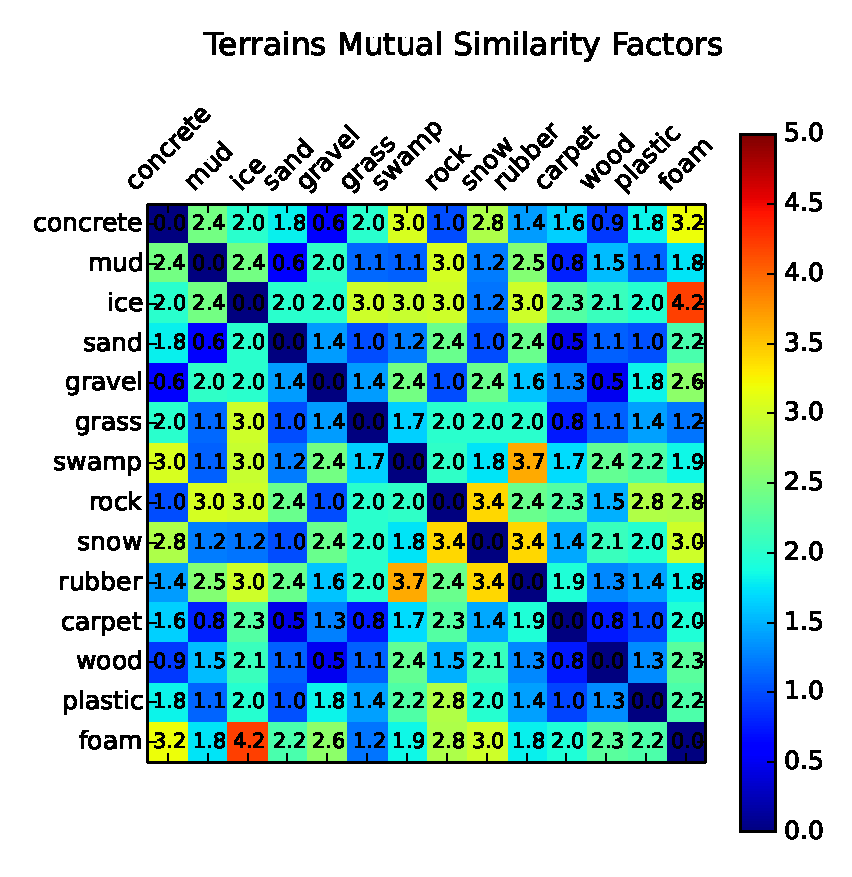
\includegraphics[width=0.8\textwidth]{terrains_variability}
  \caption{Similarity measures among various terrain types.}
  \label{fig:terrain_similarity_measures}
\end{figure}

The surfaces have been generated virtually and their similarity to real world terrains has not been verified. However, the results demonstrate that foam is very different from ice or, for instance, sand is quite similar to mud. A low similarity measure can be seen among concrete, carpet and rubber as all of them are moreless flat.

Surprisingly, a wooden terrain ended up as very similar to gravel and carpet, but a limited number of simulated terrain features have to be considered. 
On the other hand, rubber seems to be very different from swamp and snow, which is a positive outcome. Also the high grass-ice or rock-snow similarity measures make sense. 

\section{Complete Sensory Data} \label{sec:complete_sensory_data}

\begin{figure}[H]
\centering
\begin{subfigure}{0.48\textwidth}
  \centering
  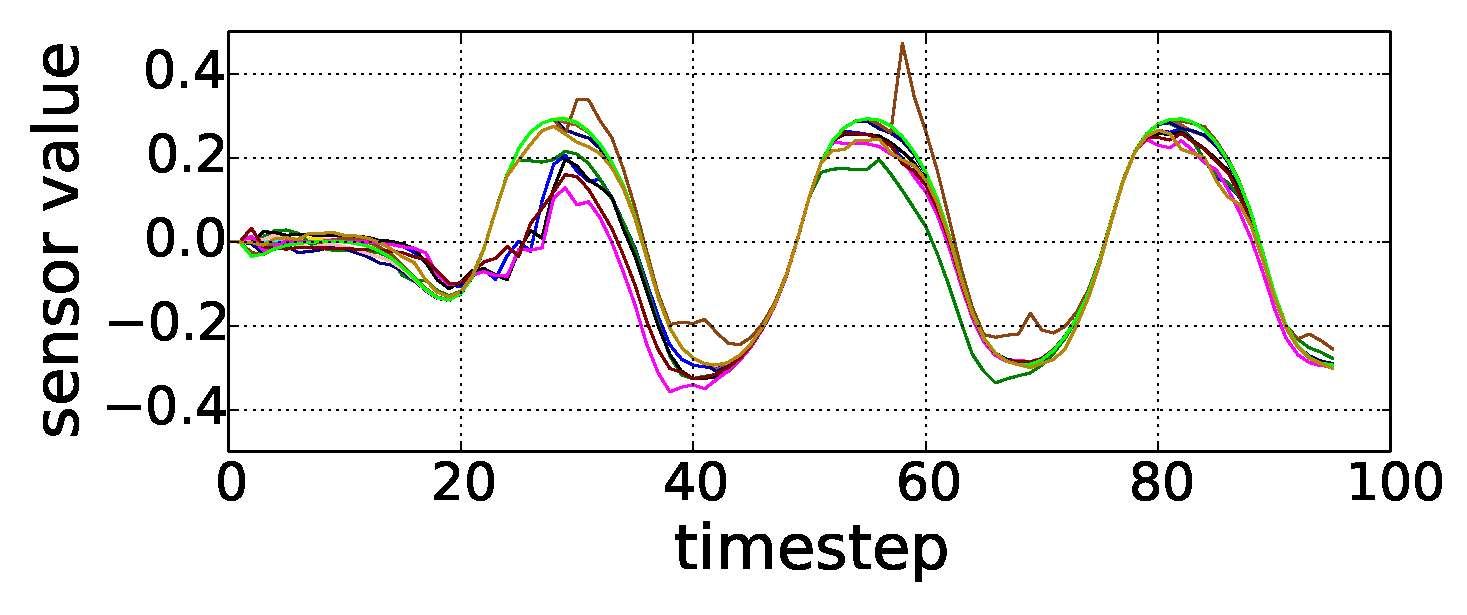
\includegraphics[width=1.0\linewidth]{app_sensor_atr_f}
  \caption{ATRf}
  \label{fig:app_atr_f}
\end{subfigure}
\begin{subfigure}{0.48\textwidth}
  \centering
  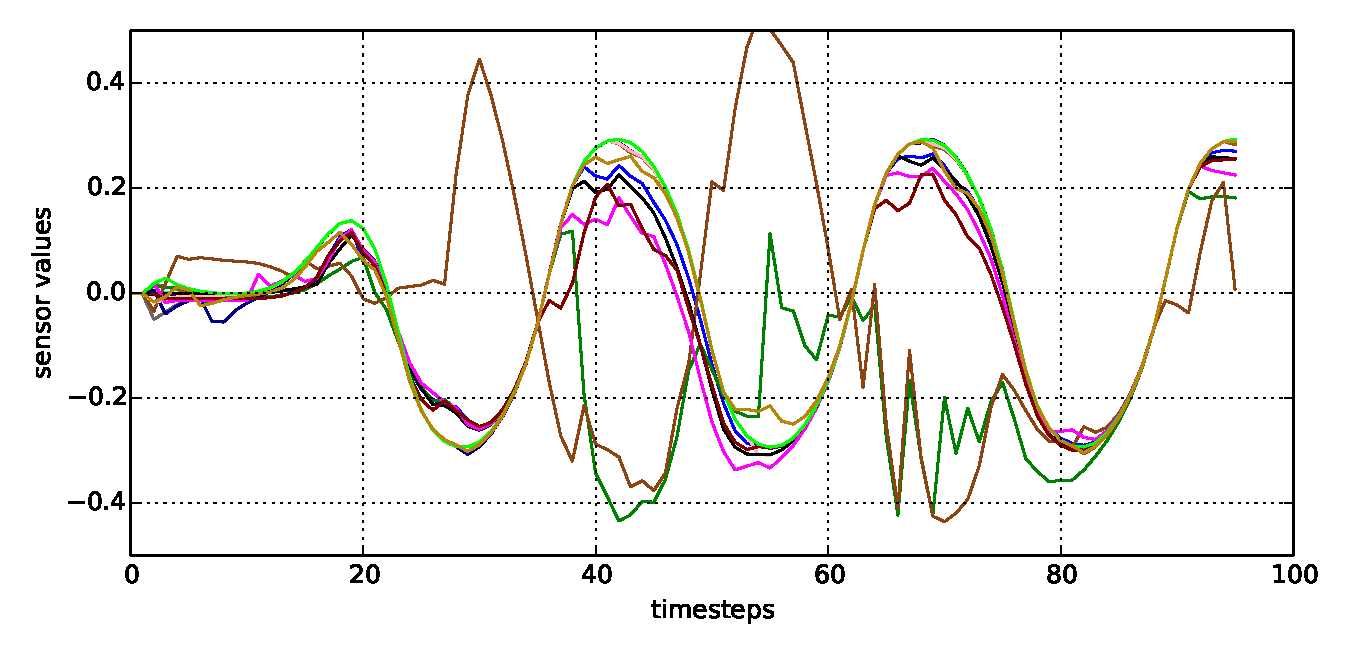
\includegraphics[width=1.0\linewidth]{app_sensor_atl_f}
  \caption{ATLf}
  \label{fig:app_atl_f}
\end{subfigure}
\caption{Thoraco joints on the front legs}
\label{fig:app_at_f}
\end{figure}

\begin{figure}[H]
\centering
\begin{subfigure}{0.48\textwidth}
  \centering
  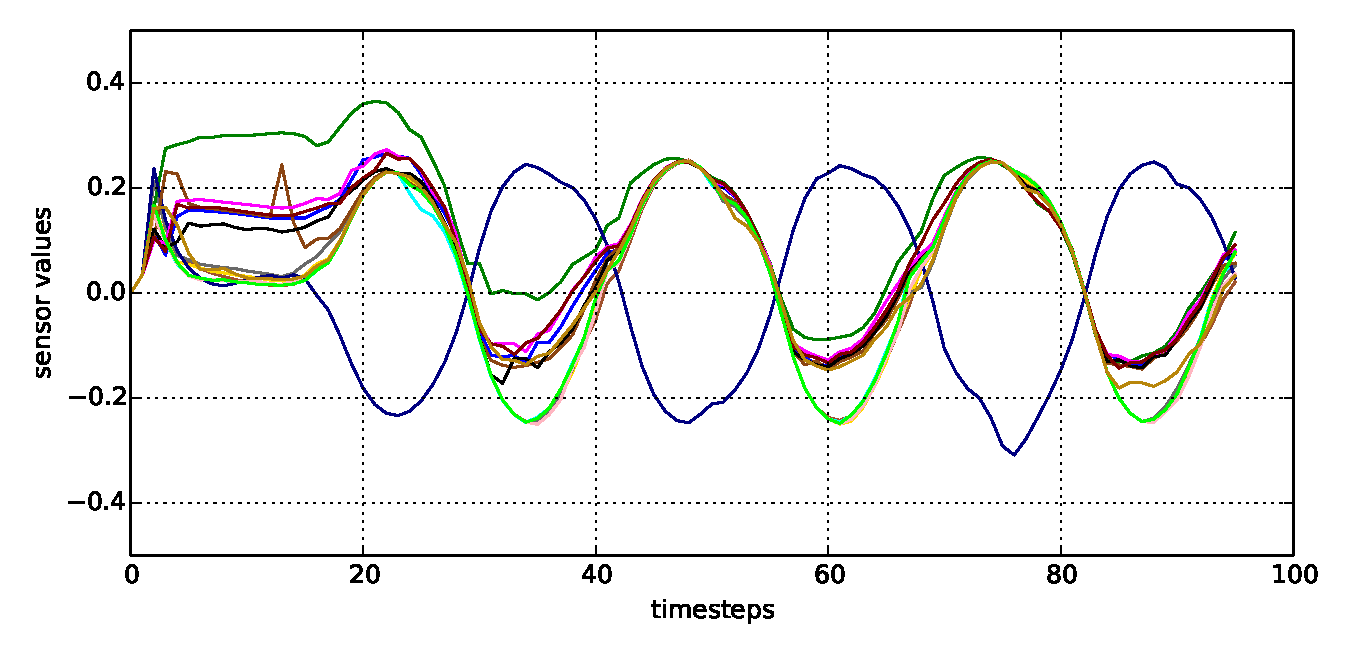
\includegraphics[width=1.0\linewidth]{app_sensor_acr_f}
  \caption{ACRf}
  \label{fig:app_acr_f}
\end{subfigure}
\begin{subfigure}{0.48\textwidth}
  \centering
  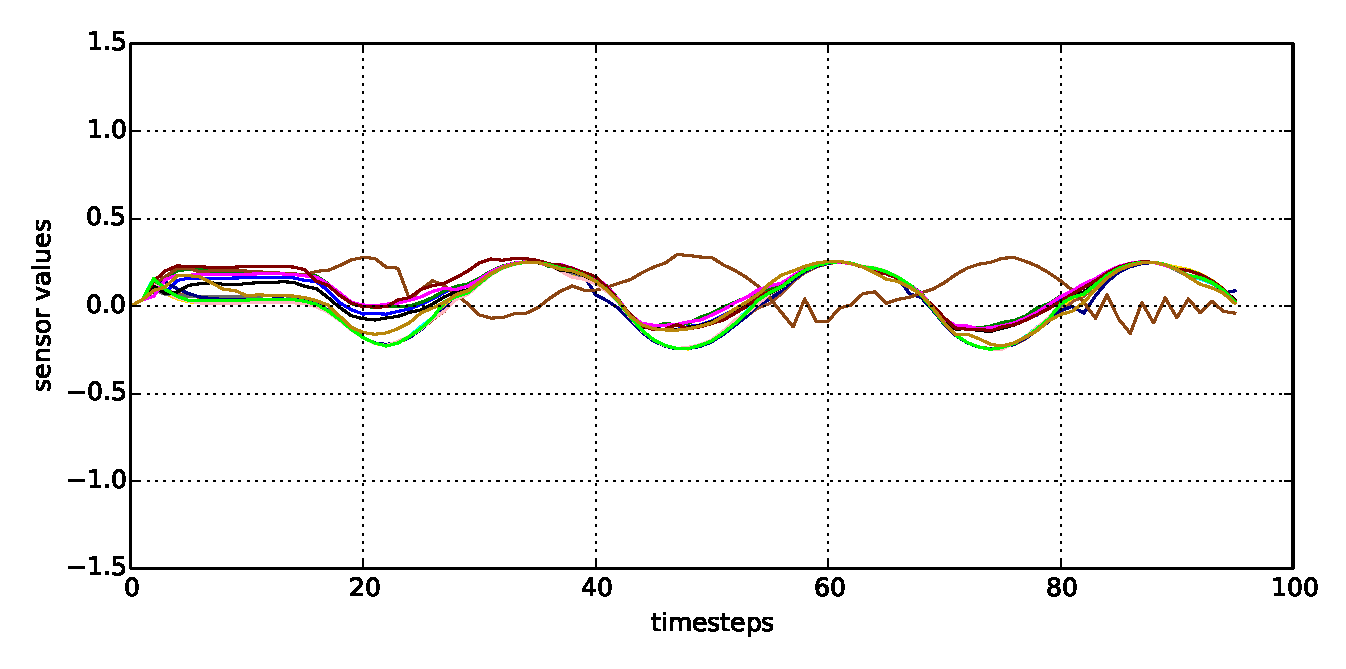
\includegraphics[width=1.0\linewidth]{app_sensor_acl_f}
  \caption{ACLf}
  \label{fig:app_acl_f}
\end{subfigure}
\caption{Coxa joints on the front legs}
\label{fig:app_ac_f}
\end{figure}

\begin{figure}[H]
\centering
\begin{subfigure}{0.48\textwidth}
  \centering
  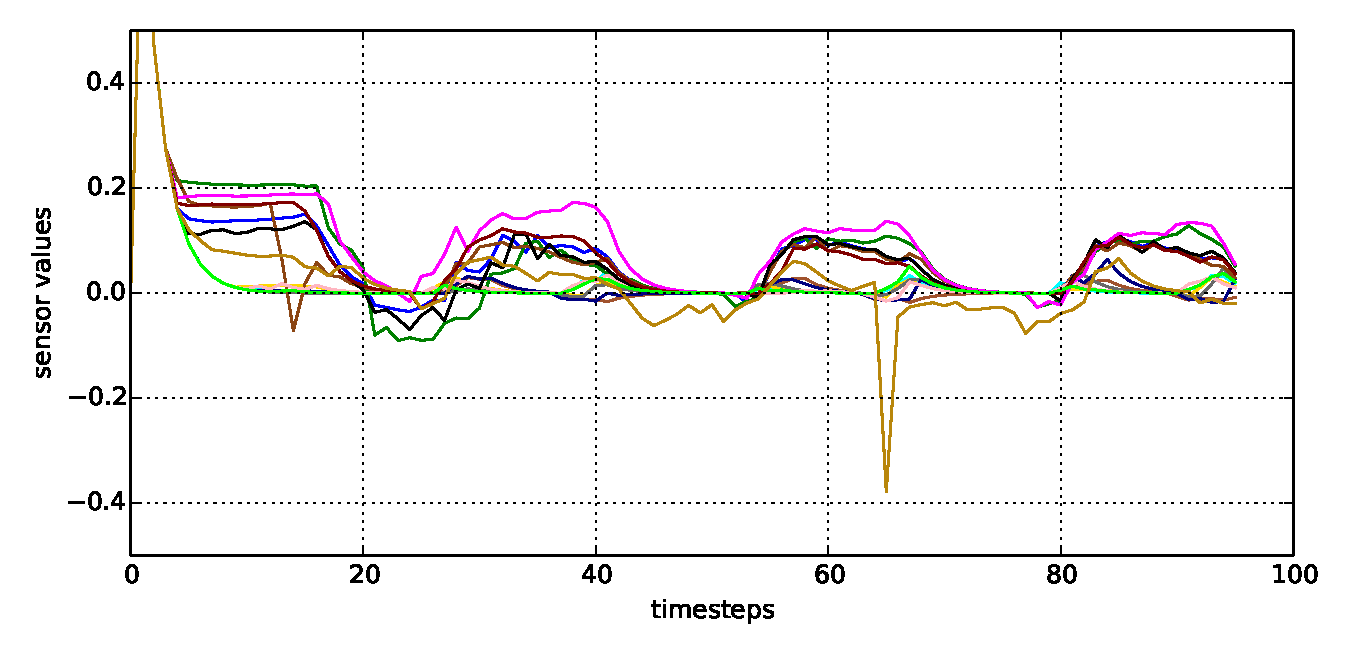
\includegraphics[width=1.0\linewidth]{app_sensor_afr_f}
  \caption{AFRf}
  \label{fig:app_afr_f}
\end{subfigure}
\begin{subfigure}{0.48\textwidth}
  \centering
  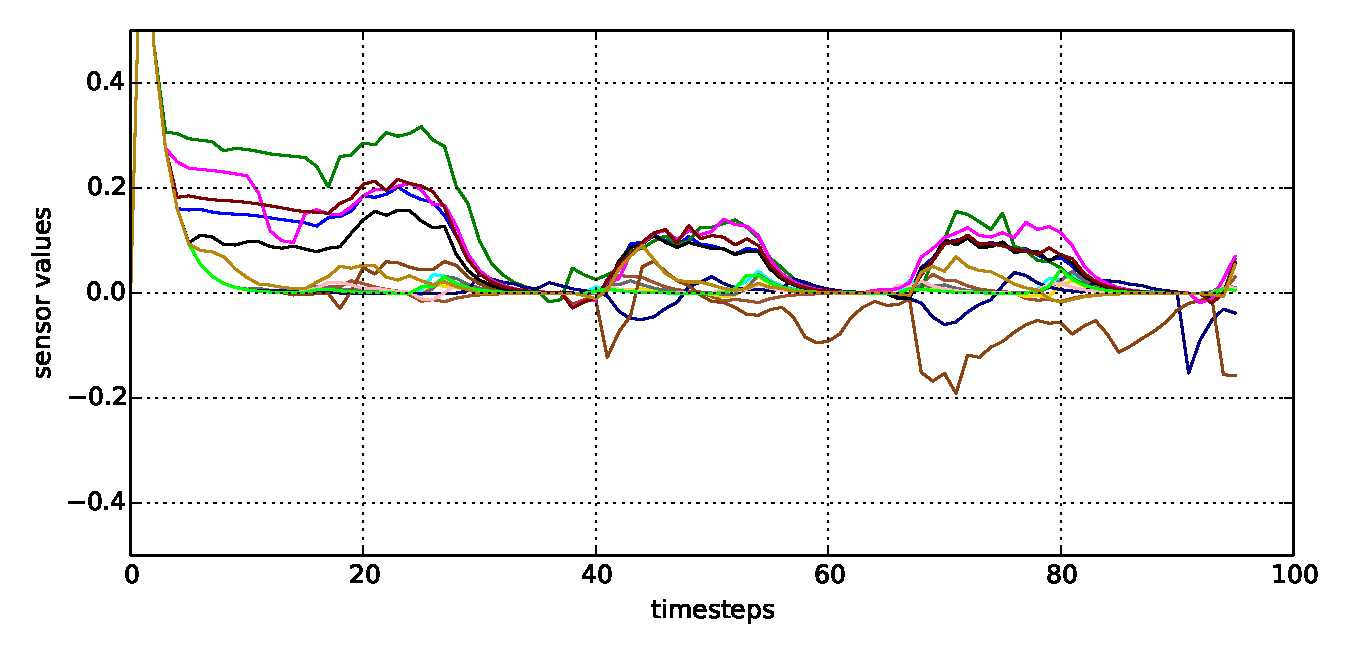
\includegraphics[width=1.0\linewidth]{app_sensor_afl_f}
  \caption{AFLf}
  \label{fig:app_afl_f}
\end{subfigure}
\caption{Femur joints on the front legs}
\label{fig:app_af_f}
\end{figure}

\begin{figure}[H]
\centering
\begin{subfigure}{0.48\textwidth}
  \centering
  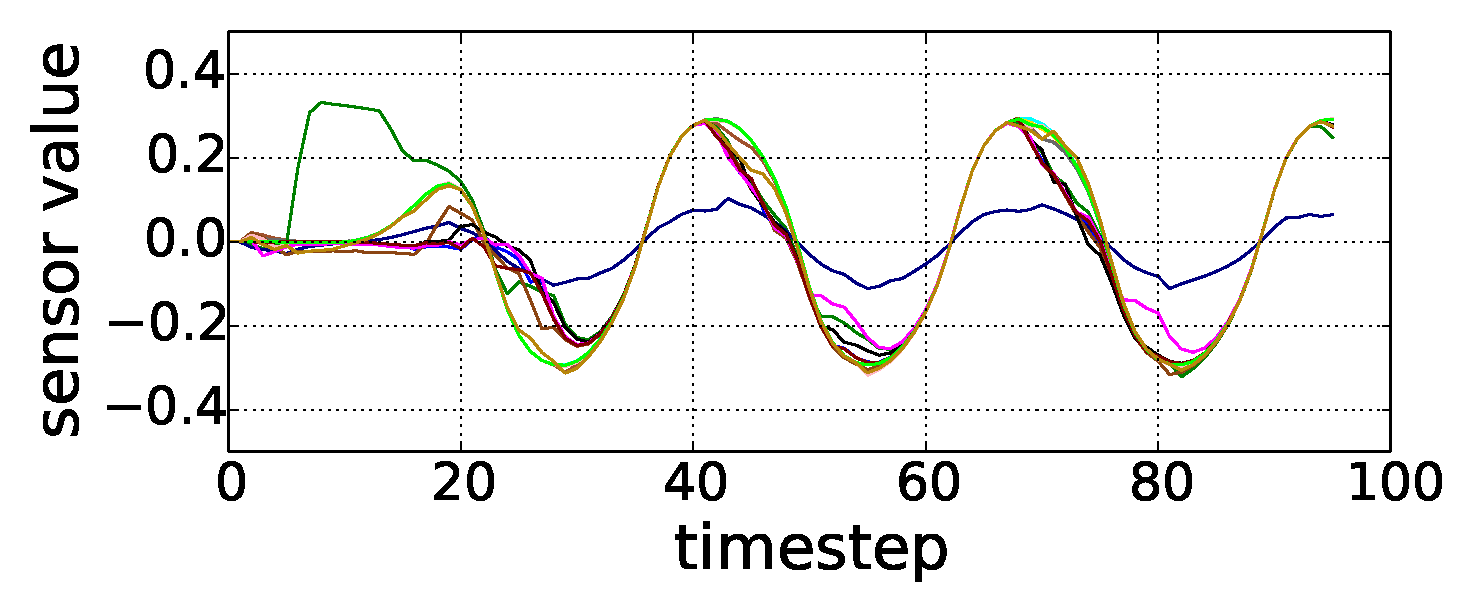
\includegraphics[width=1.0\linewidth]{app_sensor_atr_m}
  \caption{ATRm}
  \label{fig:app_atr_m}
\end{subfigure}
\begin{subfigure}{0.48\textwidth}
  \centering
  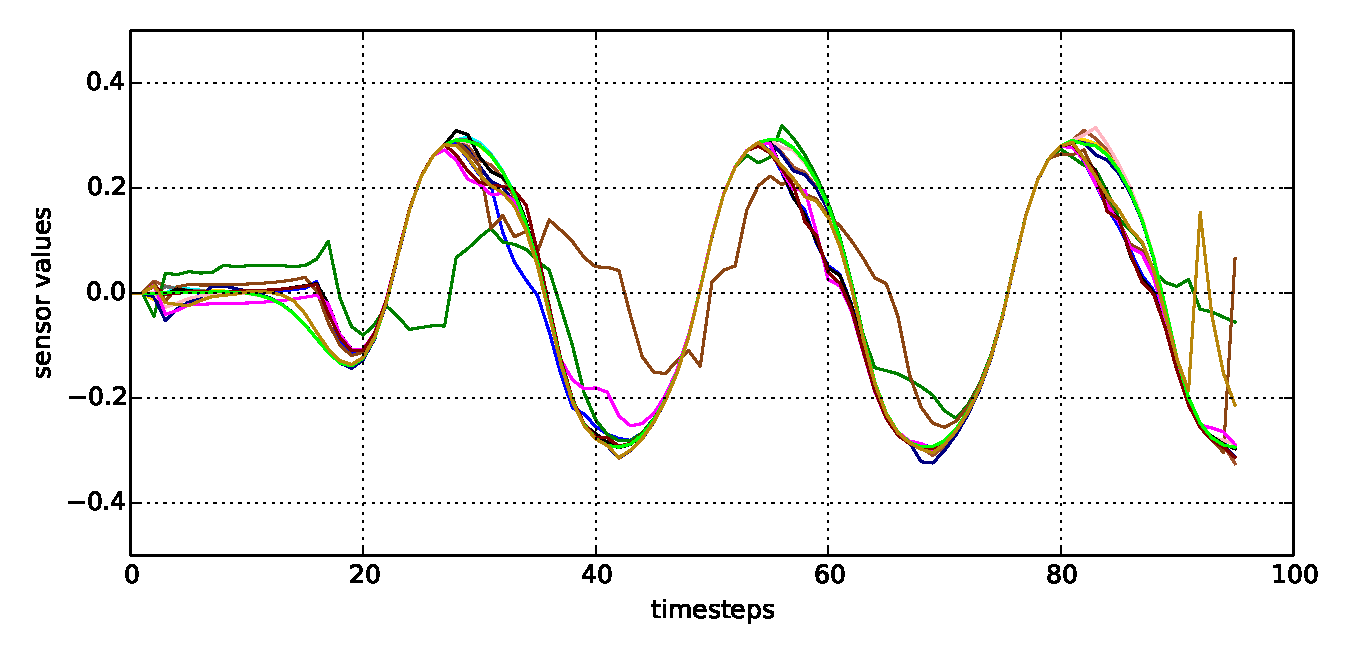
\includegraphics[width=1.0\linewidth]{app_sensor_atl_m}
  \caption{ATLm}
  \label{fig:app_atl_m}
\end{subfigure}
\caption{Thoraco joints on the middle legs}
\label{fig:app_at_m}
\end{figure}

\begin{figure}[H]
\centering
\begin{subfigure}{0.48\textwidth}
  \centering
  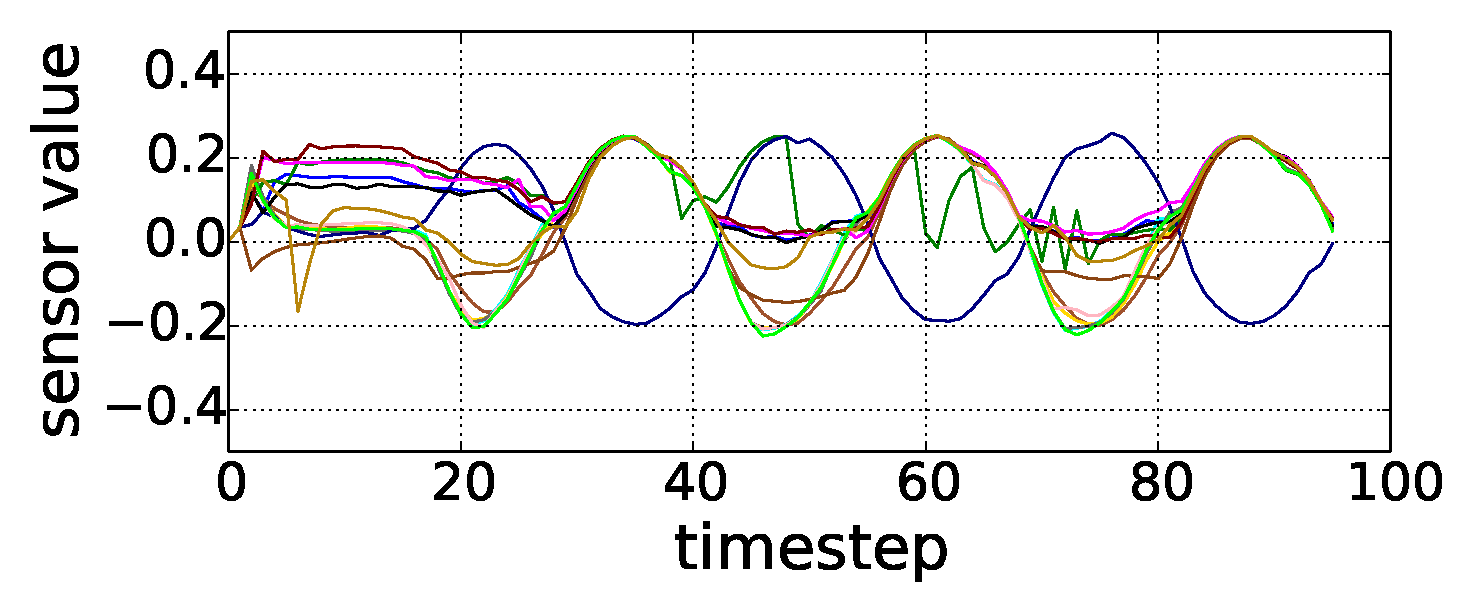
\includegraphics[width=1.0\linewidth]{app_sensor_acr_m}
  \caption{ACRm}
  \label{fig:app_acr_m}
\end{subfigure}
\begin{subfigure}{0.48\textwidth}
  \centering
  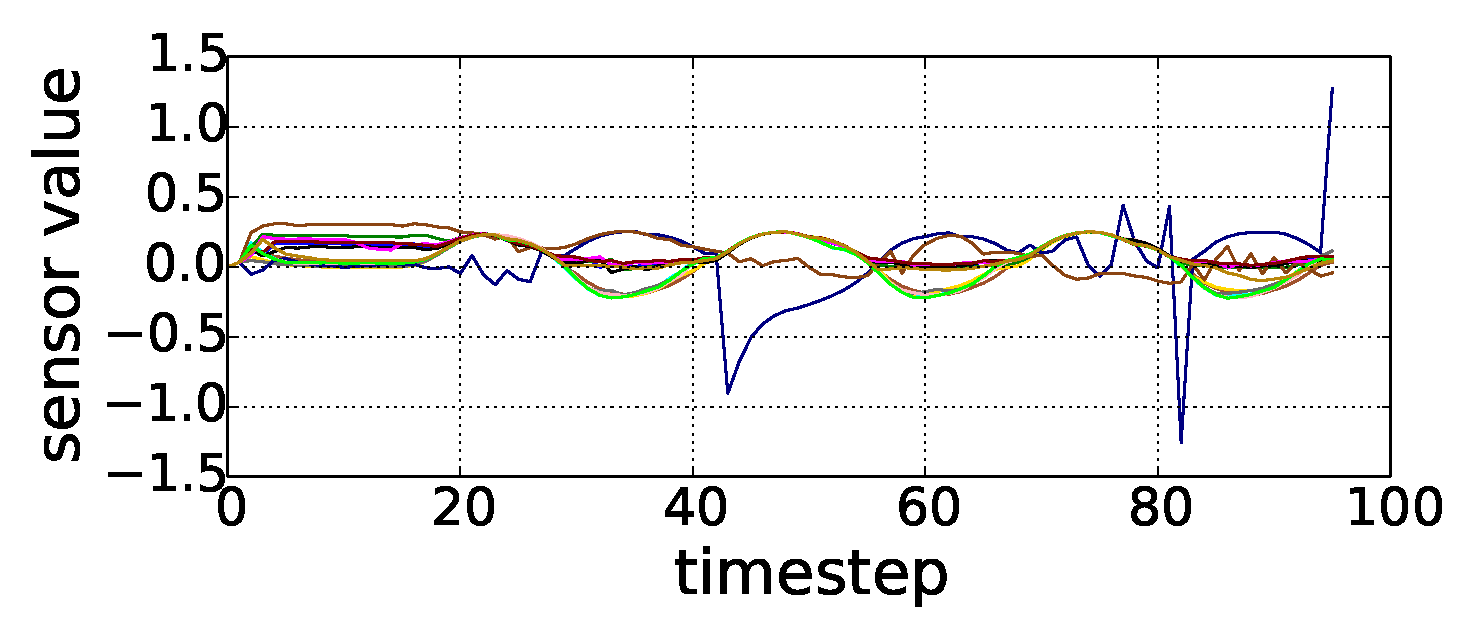
\includegraphics[width=1.0\linewidth]{app_sensor_acl_m}
  \caption{ACLm}
  \label{fig:app_acl_m}
\end{subfigure}
\caption{Coxa joints on the middle legs}
\label{fig:app_ac_m}
\end{figure}

\begin{figure}[H]
\centering
\begin{subfigure}{0.48\textwidth}
  \centering
  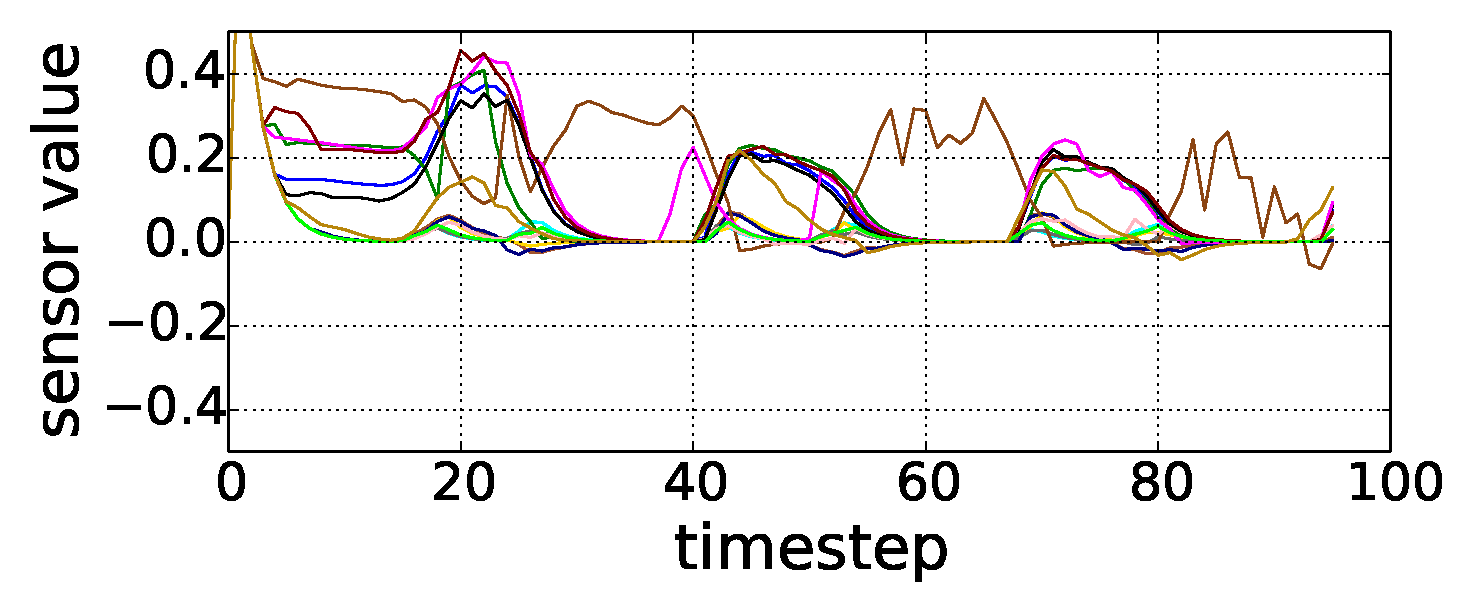
\includegraphics[width=1.0\linewidth]{app_sensor_afr_m}
  \caption{AFRm}
  \label{fig:app_afr_m}
\end{subfigure}
\begin{subfigure}{0.48\textwidth}
  \centering
  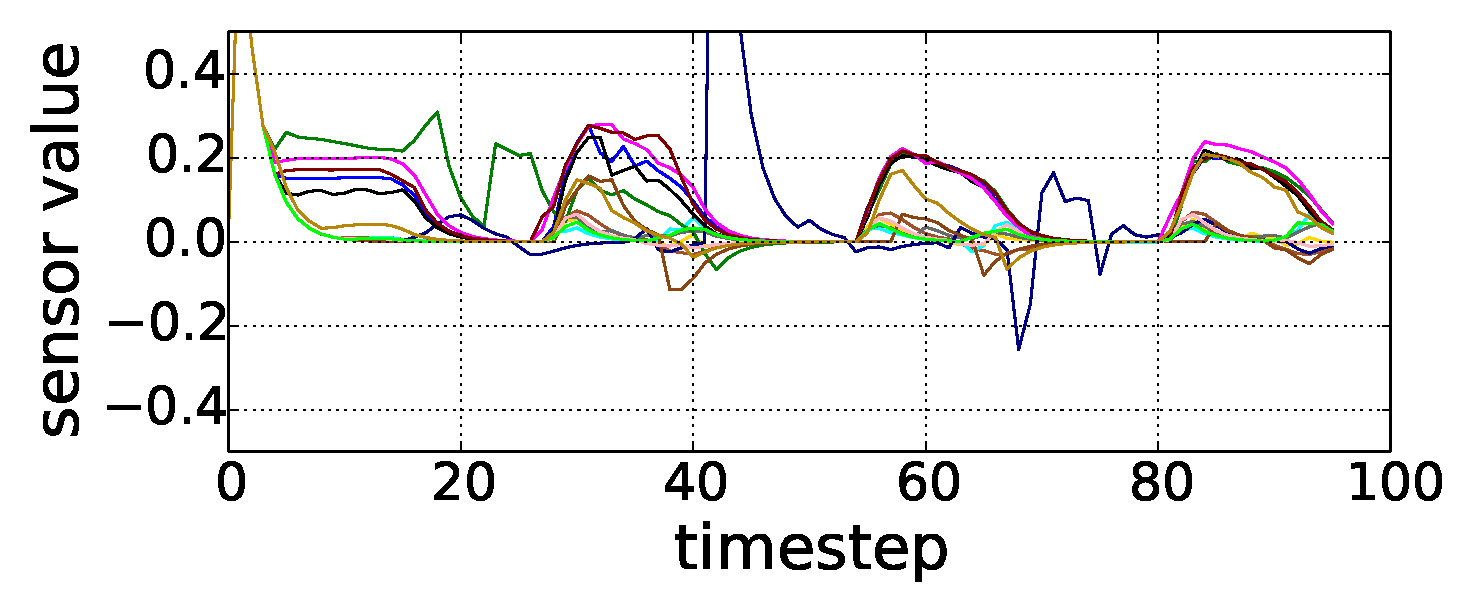
\includegraphics[width=1.0\linewidth]{app_sensor_afl_m}
  \caption{AFLm}
  \label{fig:app_afl_m}
\end{subfigure}
\caption{Thoraco joints on the middle legs}
\label{fig:app_af_m}
\end{figure}

\begin{figure}[H]
\centering
\begin{subfigure}{0.48\textwidth}
  \centering
  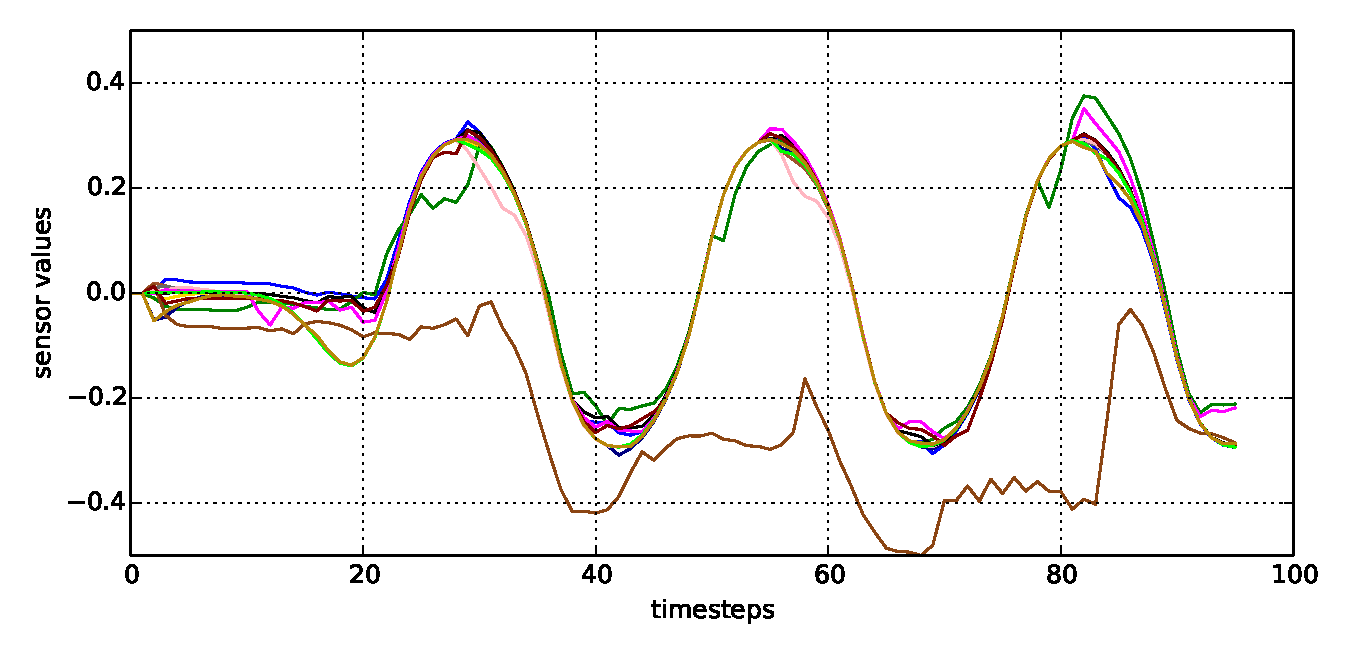
\includegraphics[width=1.0\linewidth]{app_sensor_atr_h}
  \caption{ATRh}
  \label{fig:app_atr_h}
\end{subfigure}
\begin{subfigure}{0.48\textwidth}
  \centering
  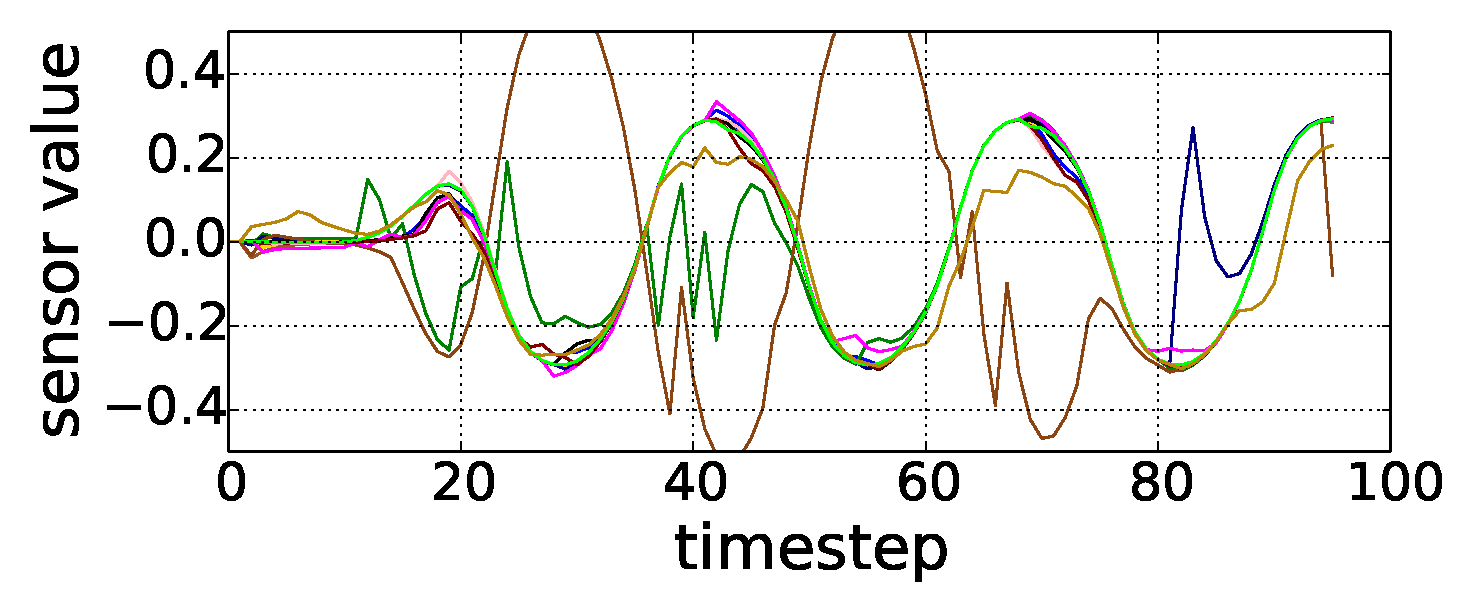
\includegraphics[width=1.0\linewidth]{app_sensor_atl_h}
  \caption{ATLh}
  \label{fig:app_atl_h}
\end{subfigure}
\caption{Thoraco joints on the hint legs}
\label{fig:app_at_h}
\end{figure}

\begin{figure}[H]
\centering
\begin{subfigure}{0.48\textwidth}
  \centering
  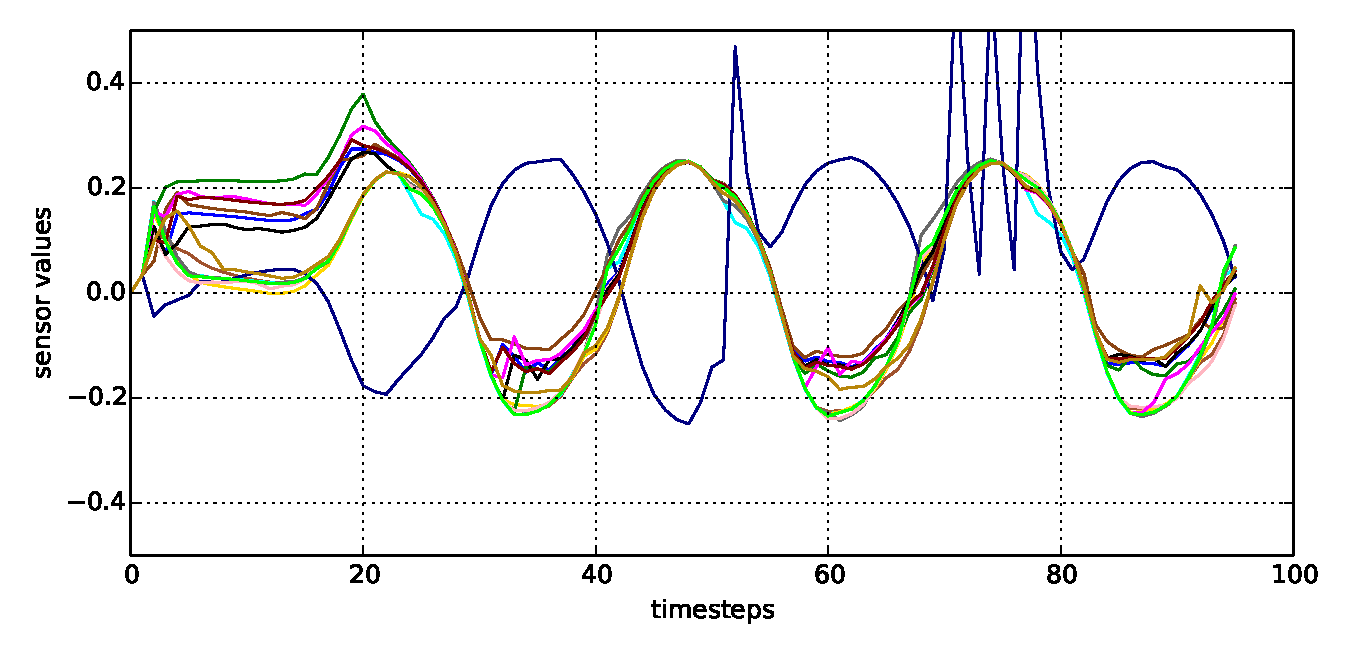
\includegraphics[width=1.0\linewidth]{app_sensor_acr_h}
  \caption{ACRh}
  \label{fig:app_acr_h}
\end{subfigure}
\begin{subfigure}{0.48\textwidth}
  \centering
  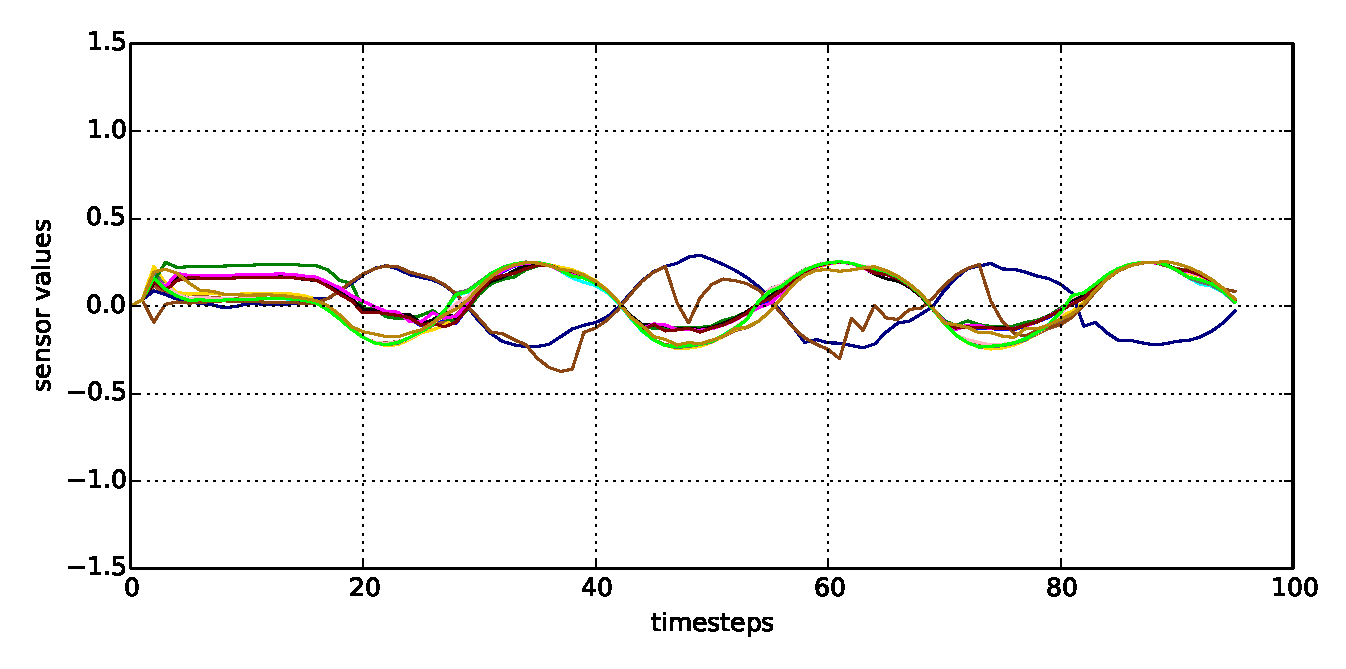
\includegraphics[width=1.0\linewidth]{app_sensor_acl_h}
  \caption{ACLh}
  \label{fig:app_acl_h}
\end{subfigure}
\caption{Coxa joints on the hint legs}
\label{fig:app_ac_h}
\end{figure}

\begin{figure}[H]
\centering
\begin{subfigure}{0.48\textwidth}
  \centering
  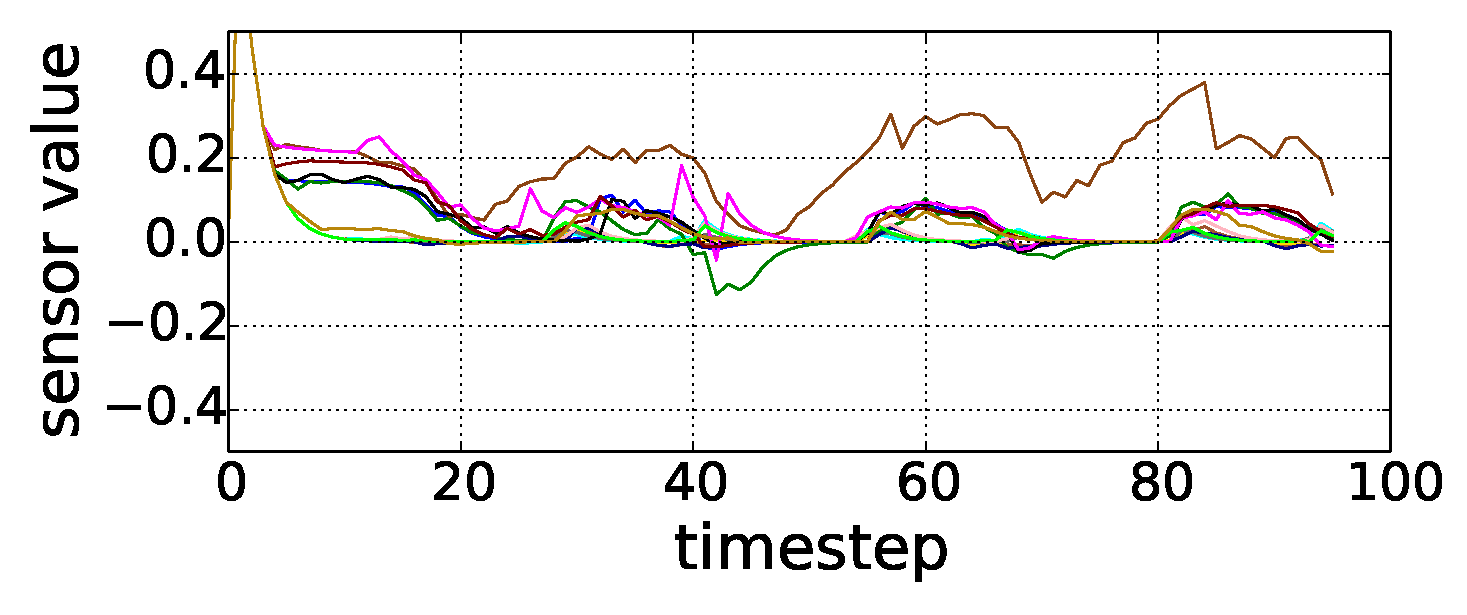
\includegraphics[width=1.0\linewidth]{app_sensor_afr_h}
  \caption{AFRh}
  \label{fig:app_afr_h}
\end{subfigure}
\begin{subfigure}{0.48\textwidth}
  \centering
  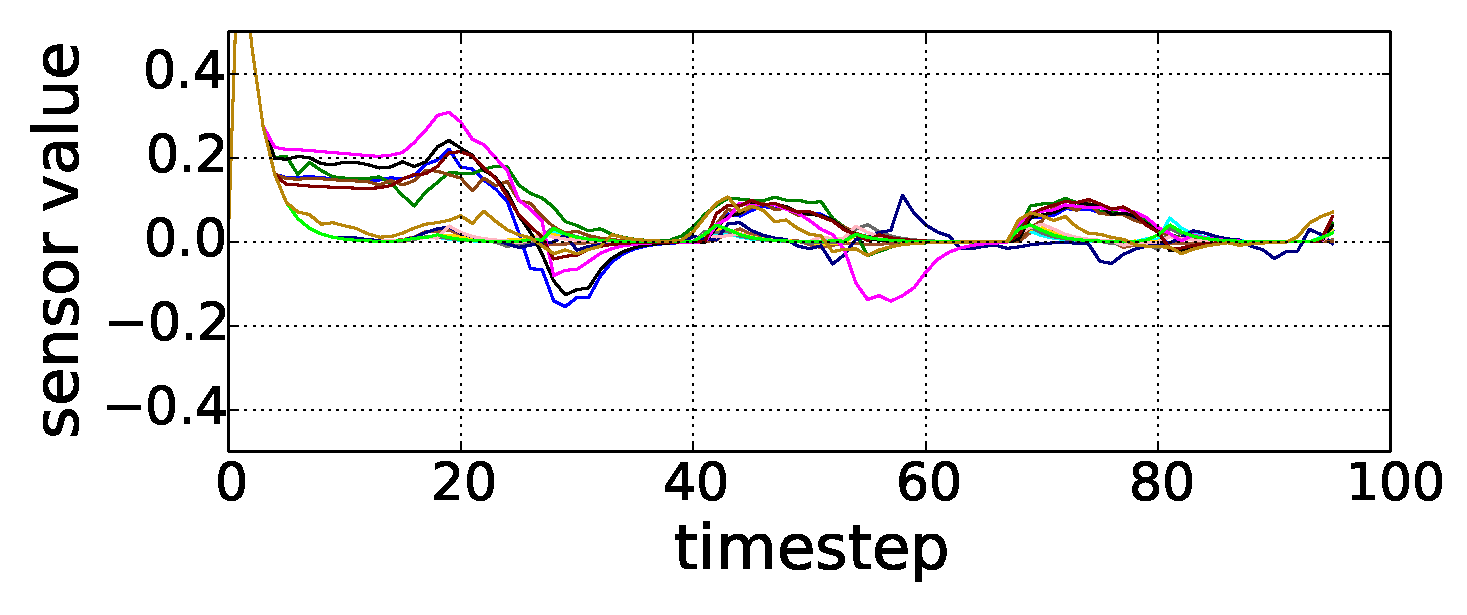
\includegraphics[width=1.0\linewidth]{app_sensor_afl_h}
  \caption{AFLh}
  \label{fig:app_afl_h}
\end{subfigure}
\caption{Thoraco joints on the hint legs}
\label{fig:app_af_h}
\end{figure}

\begin{figure}[H]
\centering
\begin{subfigure}{0.48\textwidth}
  \centering
  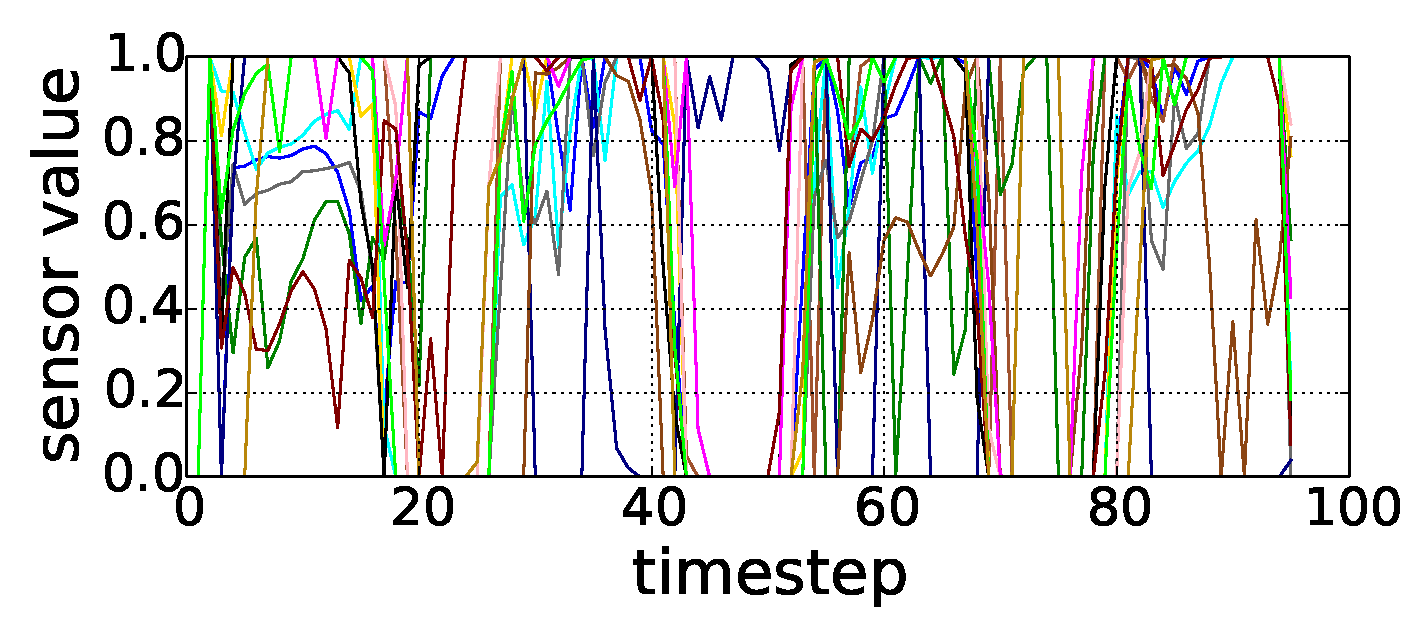
\includegraphics[width=1.0\linewidth]{app_sensor_fr_f}
  \caption{FRf}
  \label{fig:app_fr_f}
\end{subfigure}
\begin{subfigure}{0.48\textwidth}
  \centering
  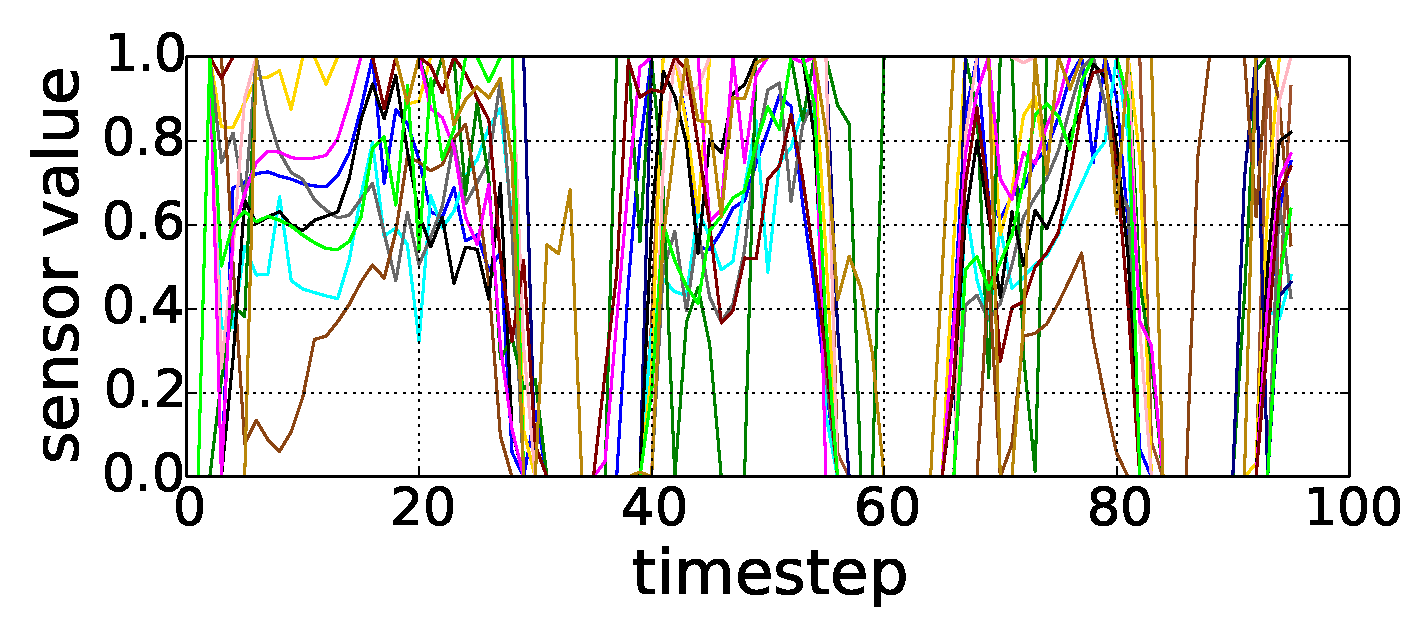
\includegraphics[width=1.0\linewidth]{app_sensor_fl_f}
  \caption{FLf}
  \label{fig:app_fl_f}
\end{subfigure}
\caption{Foot contact sensors on the front legs}
\label{fig:app_f_f}
\end{figure}

\begin{figure}[H]
\centering
\begin{subfigure}{0.48\textwidth}
  \centering
  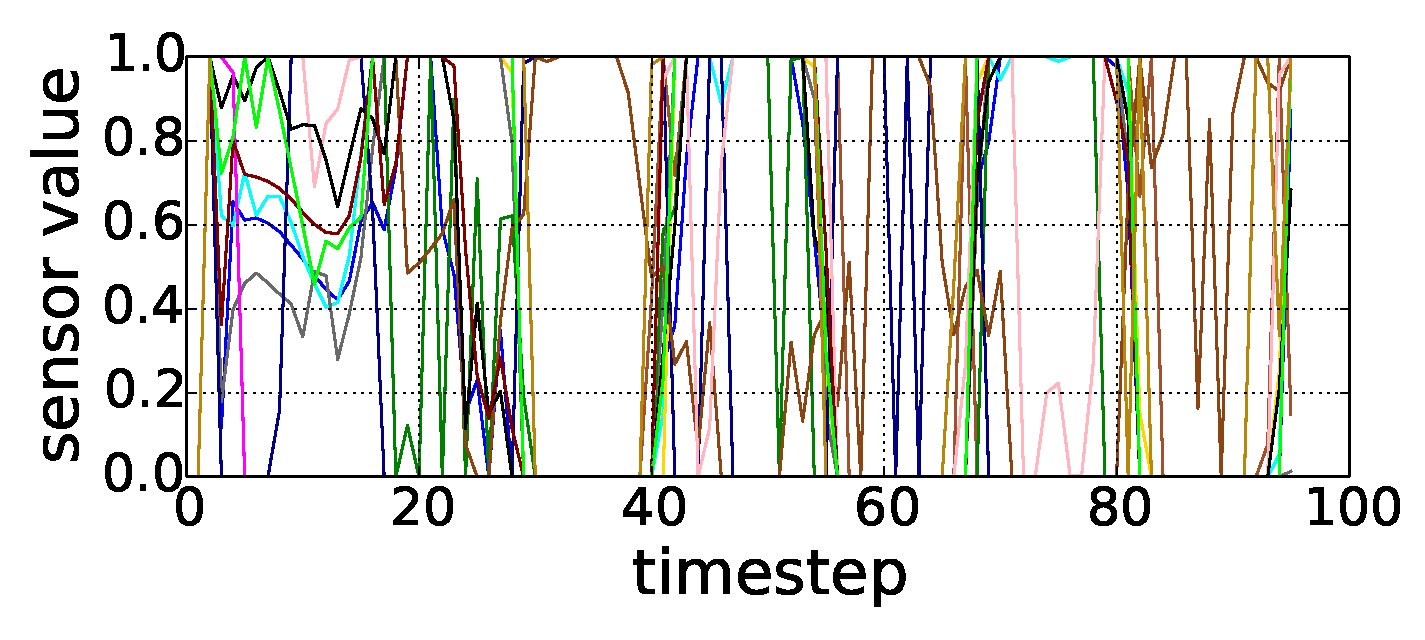
\includegraphics[width=1.0\linewidth]{app_sensor_fr_m}
  \caption{FRm}
  \label{fig:app_fr_m}
\end{subfigure}
\begin{subfigure}{0.48\textwidth}
  \centering
  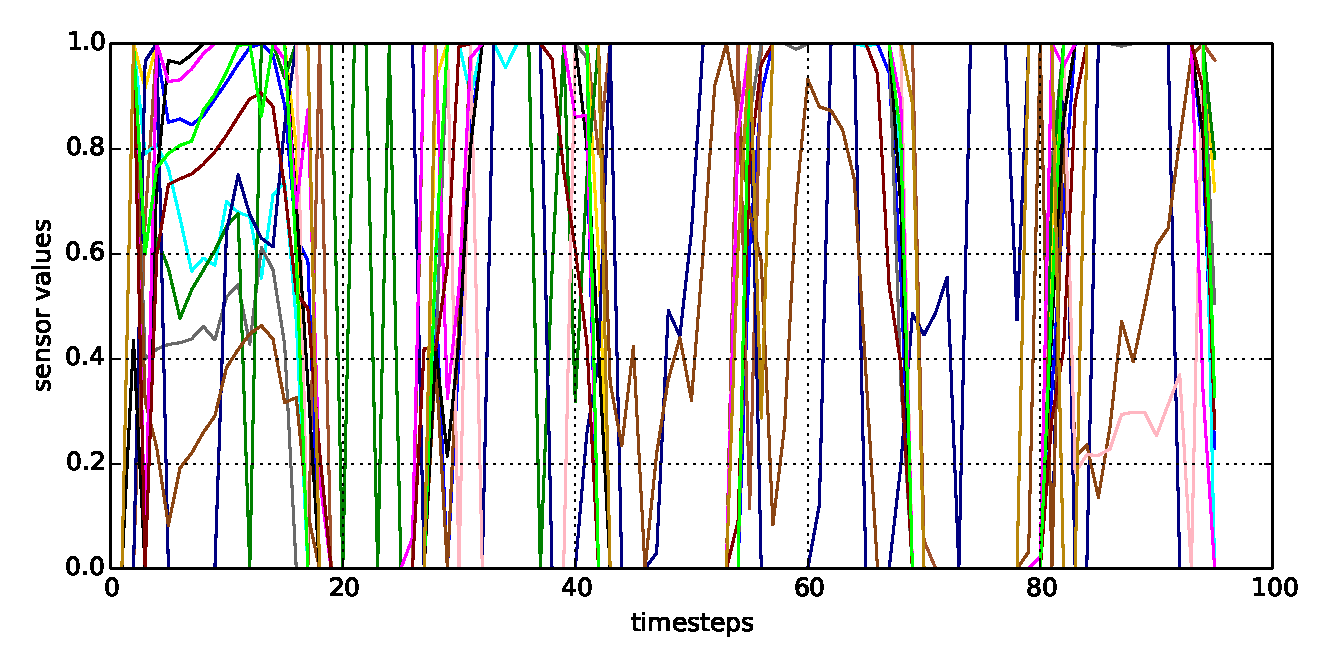
\includegraphics[width=1.0\linewidth]{app_sensor_fl_m}
  \caption{FLm}
  \label{fig:app_fl_m}
\end{subfigure}
\caption{Foot contact sensors on the middle legs}
\label{fig:app_f_m}
\end{figure}

\begin{figure}[H]
\centering
\begin{subfigure}{0.48\textwidth}
  \centering
  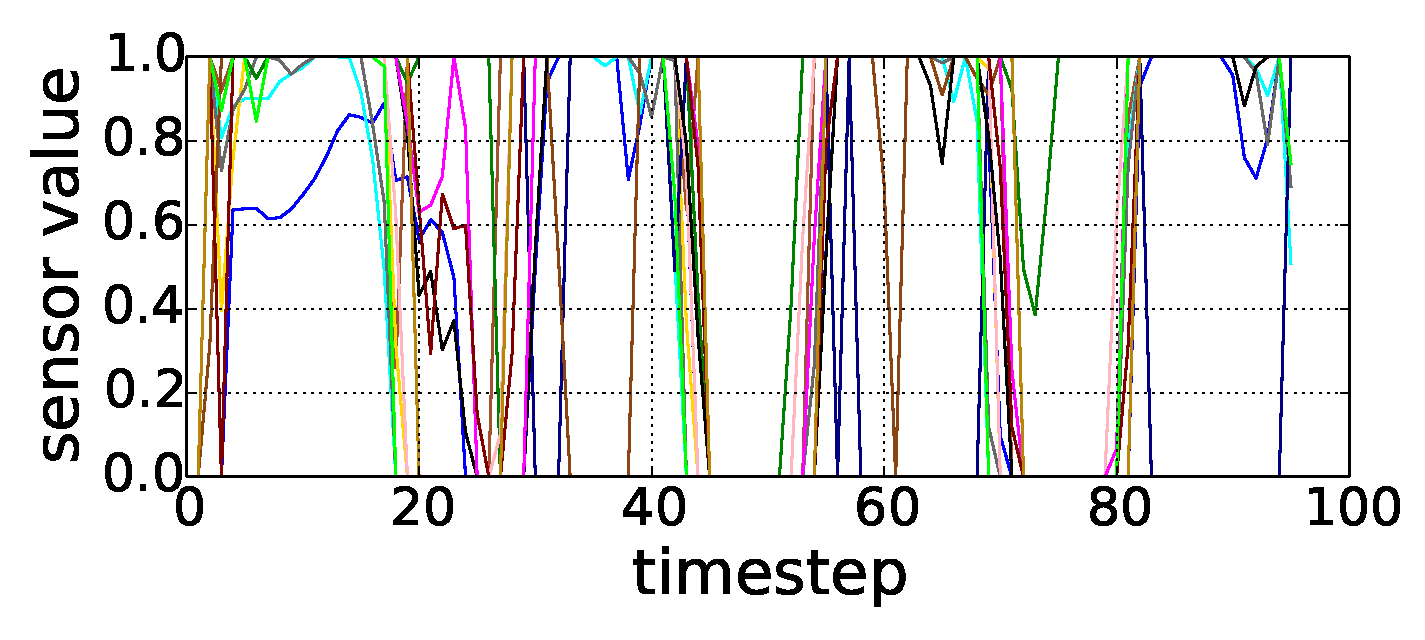
\includegraphics[width=1.0\linewidth]{app_sensor_fr_h}
  \caption{FRh}
  \label{fig:app_fr_h}
\end{subfigure}
\begin{subfigure}{0.48\textwidth}
  \centering
  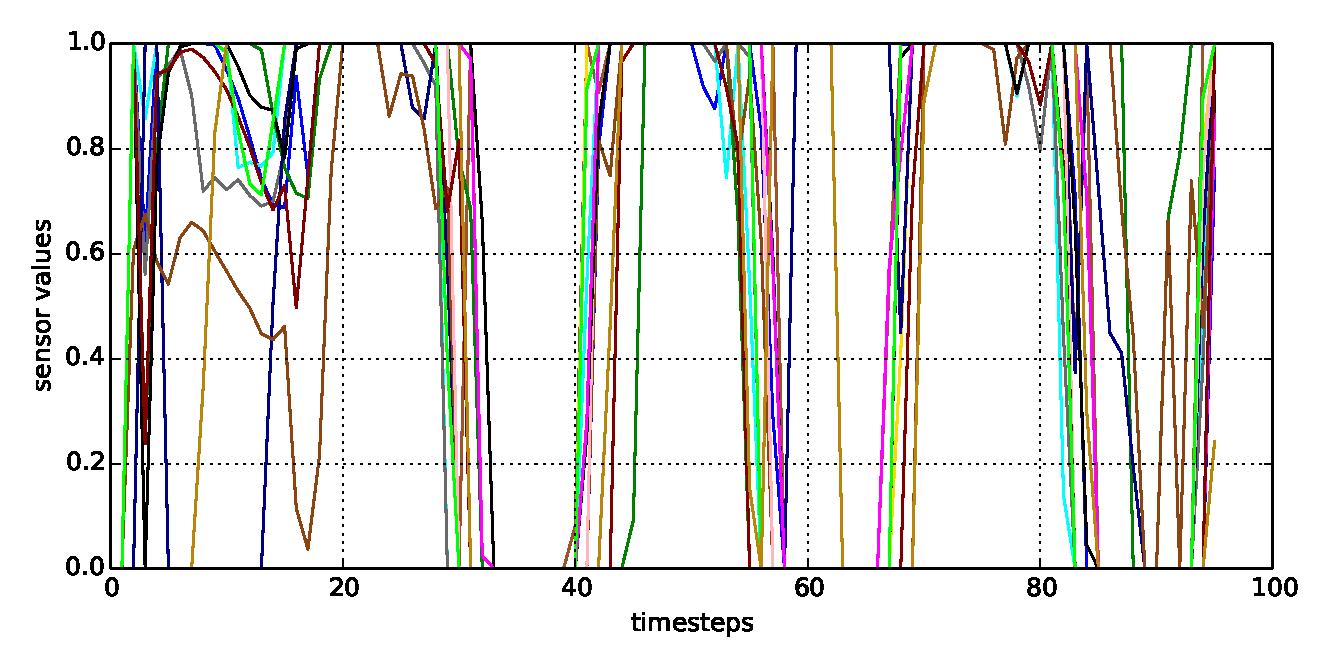
\includegraphics[width=1.0\linewidth]{app_sensor_fl_h}
  \caption{FLh}
  \label{fig:app_fl_h}
\end{subfigure}
\caption{Foot contact sensors on the hint legs}
\label{fig:app_f_h}
\end{figure}

\section{Further Data Analysis} \label{sec:further_data_analysis}

\begin{figure}[H]
  \centering
  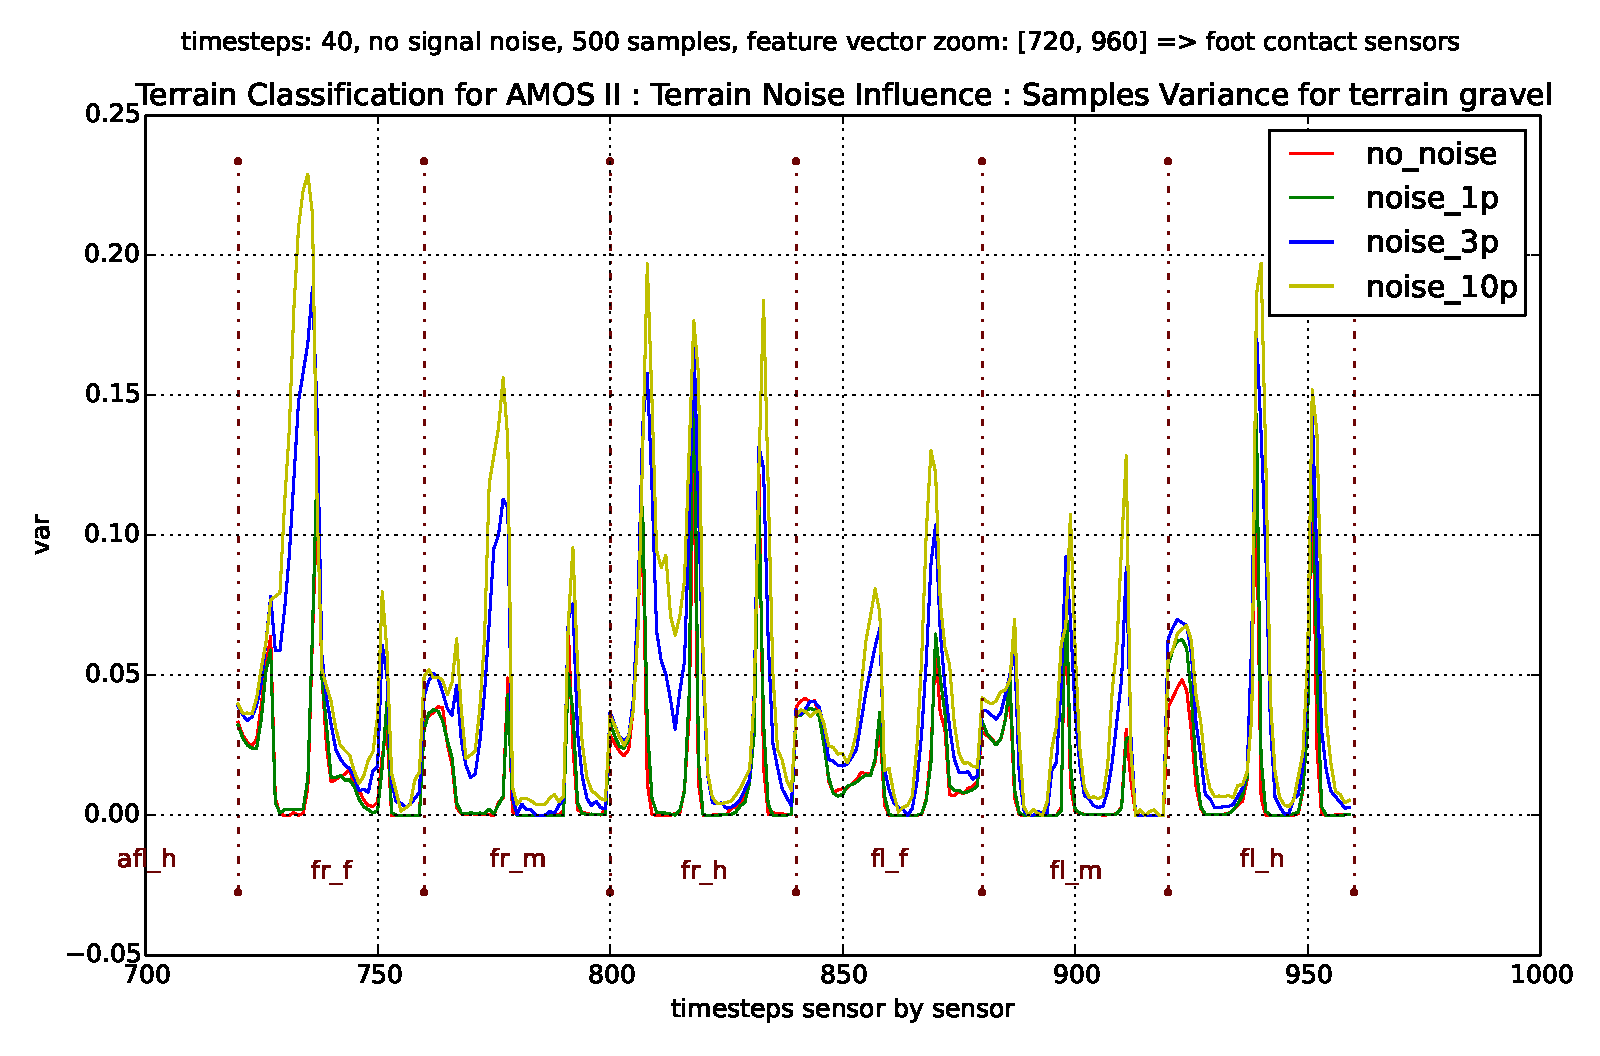
\includegraphics[width=1.0\textwidth]{tn_analysis_40_foot_contact_gravel}
  \caption{Terrain Noise Analysis (samples variance): 500 samples, terrain gravel, foot contact sensors (feature vector [720:960] for 40 timesteps)}
  \label{fig:tn_analysis_foot_contact_gravel}
\end{figure}

\begin{figure}[H]
  \centering
  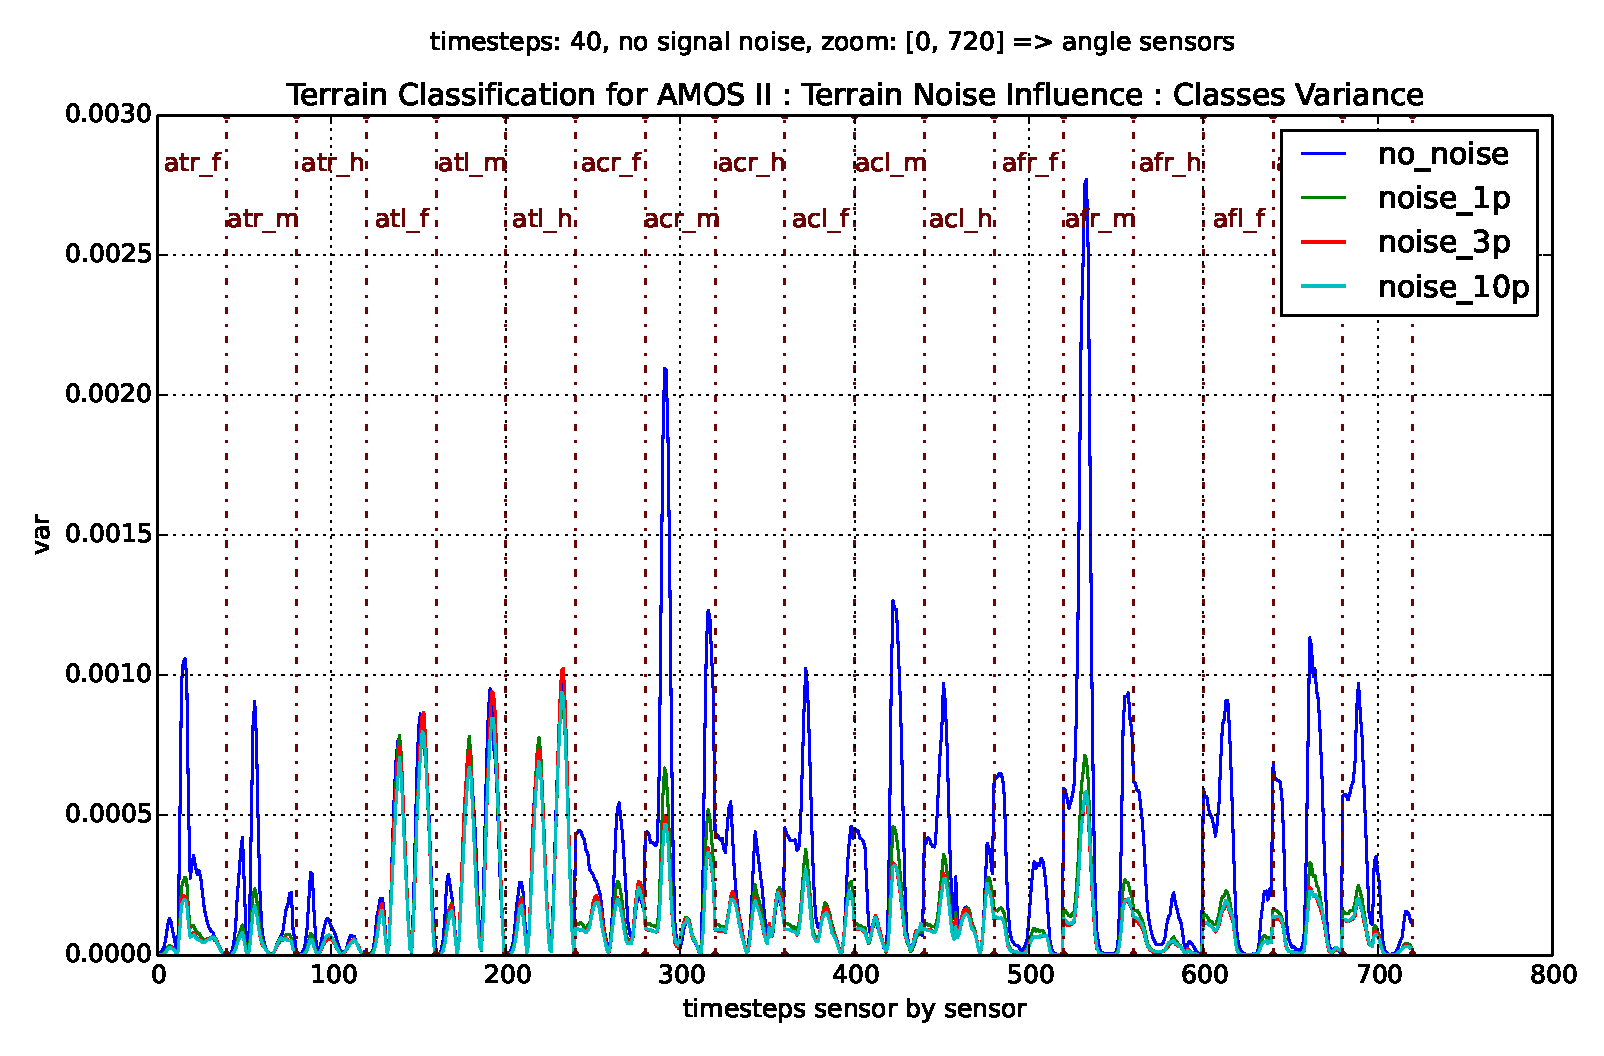
\includegraphics[width=1.0\textwidth]{tn_analysis_40_angle}
  \caption{Terrain Noise Analysis (classes variance): means of 500 samples, 14 terrains, angle sensors}
  \label{fig:tn_analysis_angle}
\end{figure}

\begin{figure}[H]
  \centering
  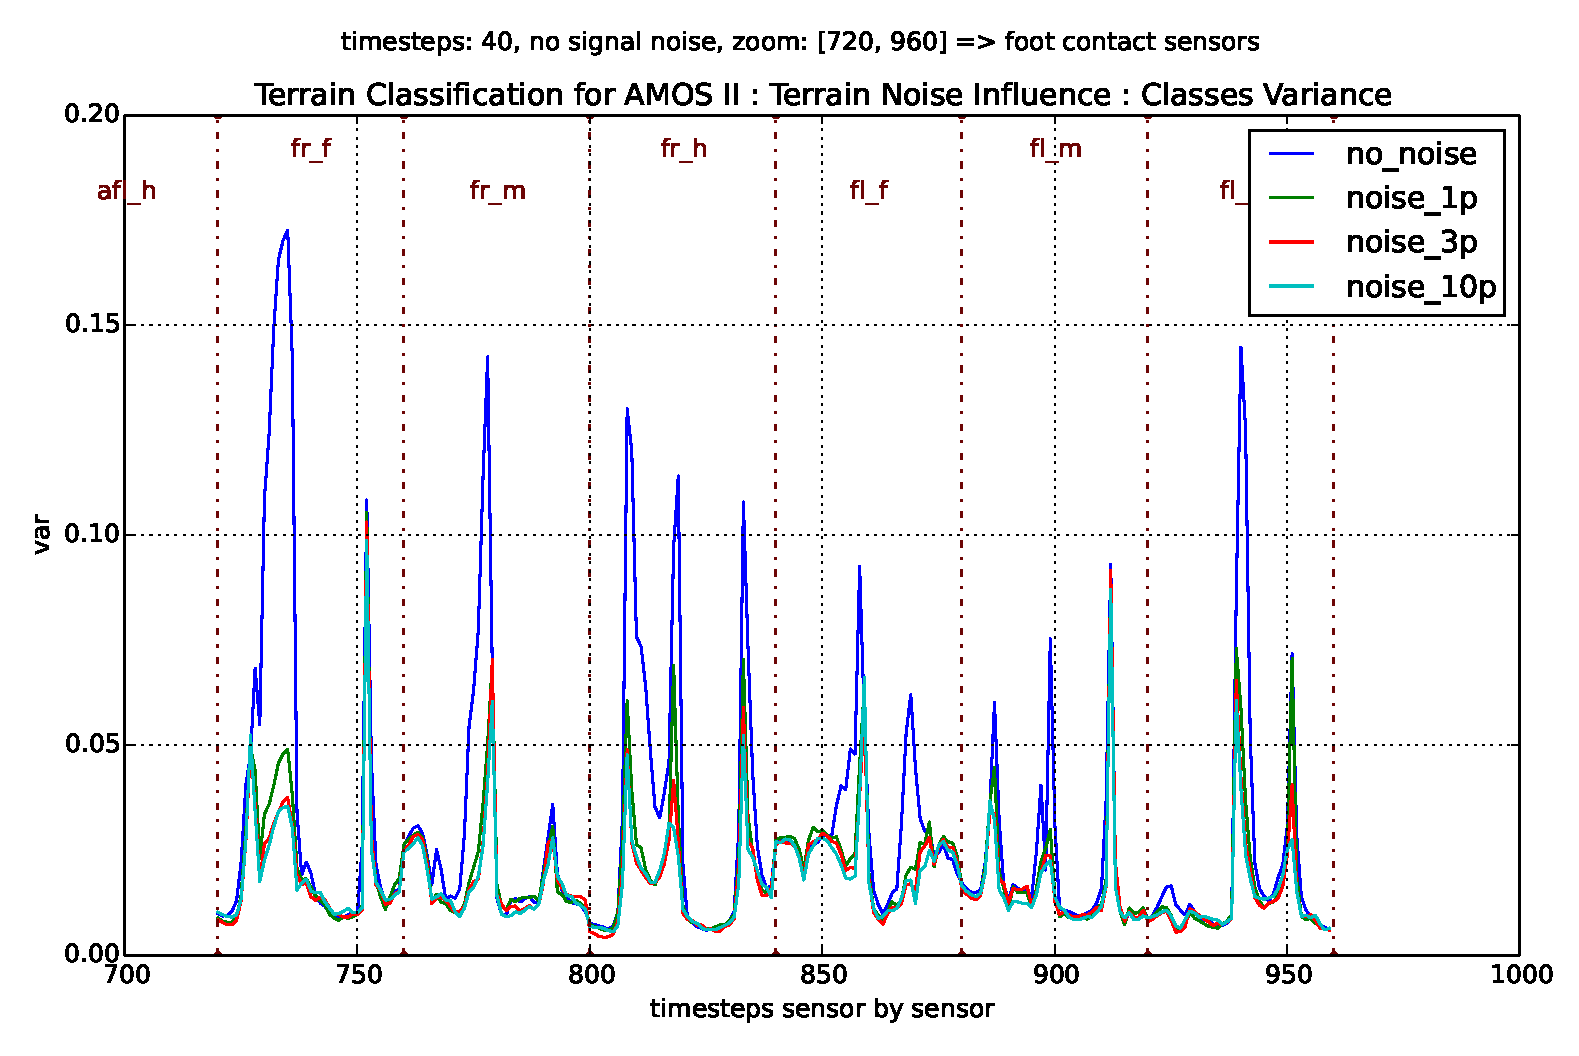
\includegraphics[width=1.0\textwidth]{tn_analysis_40_foot_contact}
  \caption{Terrain Noise Analysis (classes variance): means of 500 samples, 14 terrains, foot contact sensors}
  \label{fig:tn_analysis_foot_contact}
\end{figure}

\begin{figure}[H]
  \centering
  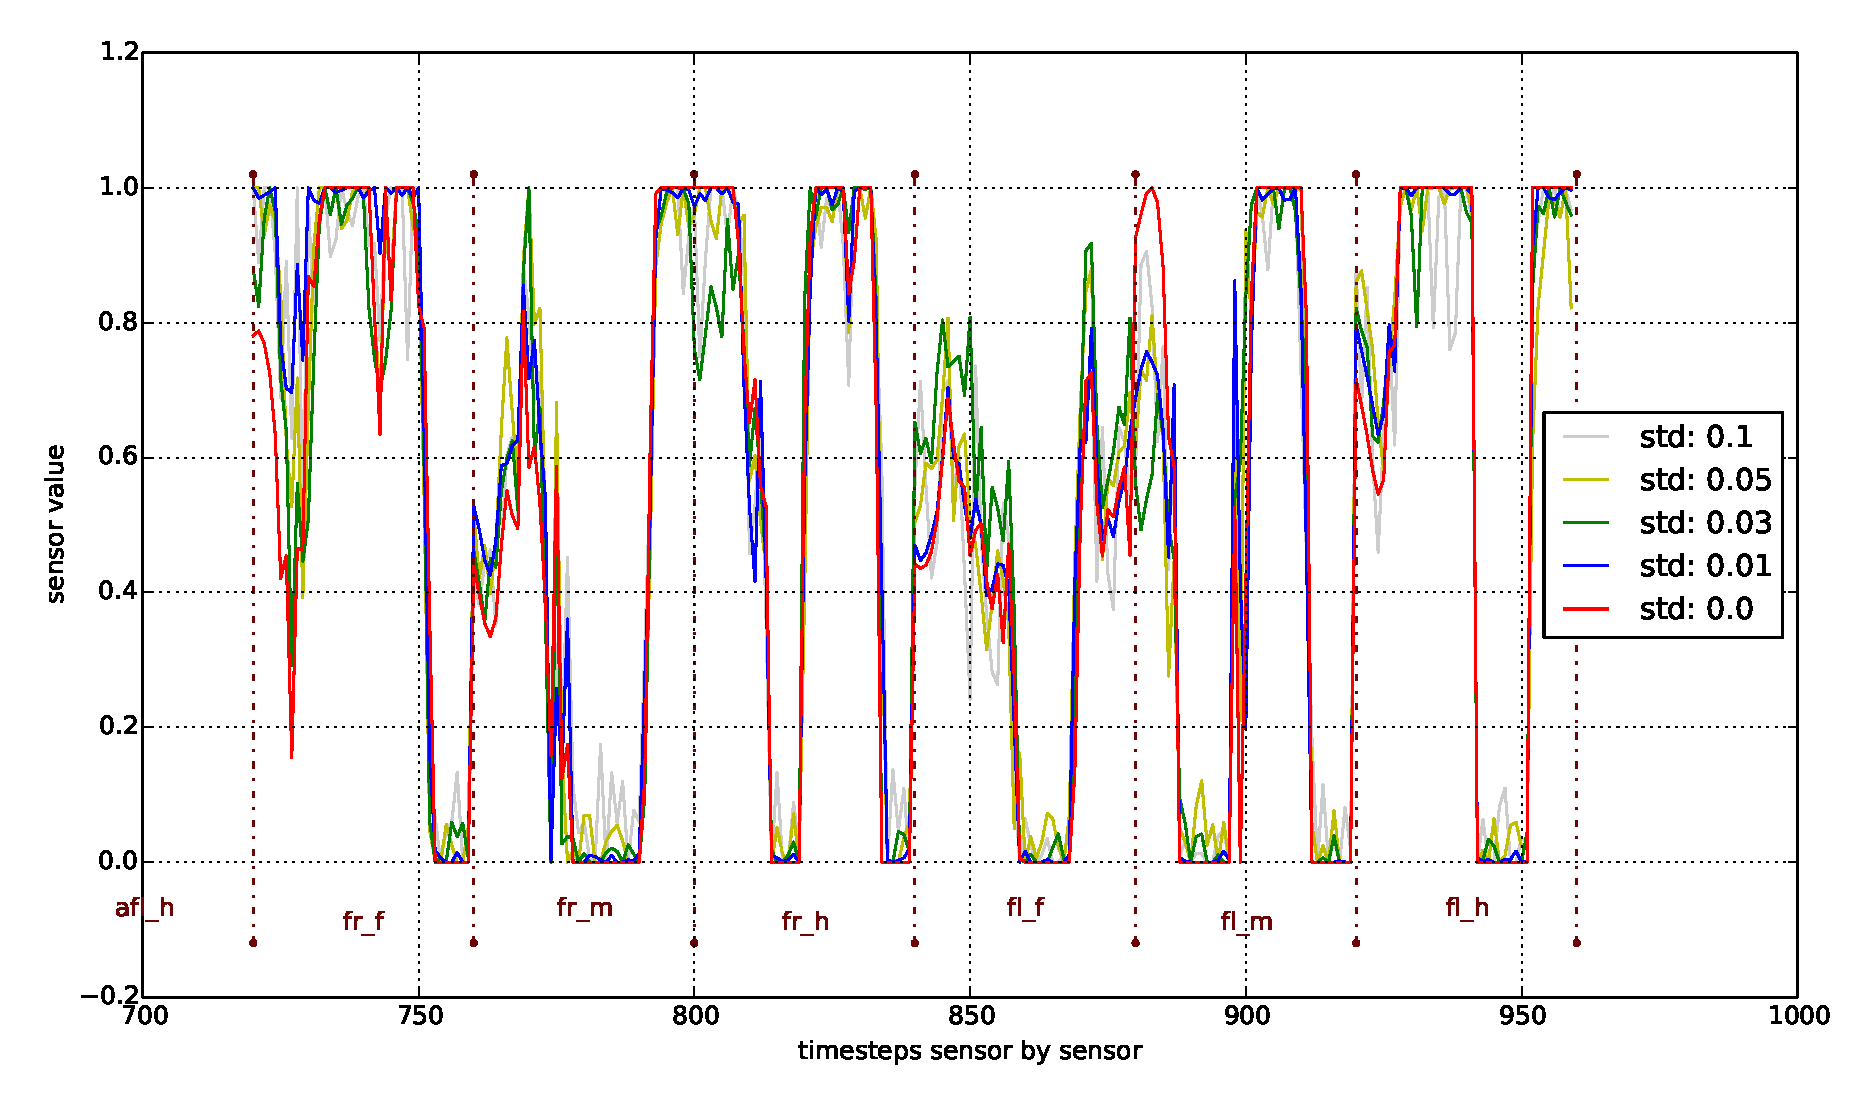
\includegraphics[width=1.0\textwidth]{sn_influence_samples_concrete_fc}
  \caption{Signal noise influence on one sample, terrain: concrete, foot contact sensors}
  \label{fig:sn_influence_samples_concrete_fc}
\end{figure}

% samples variances for signal noise
%\begin{figure}[H]
%  \centering
%  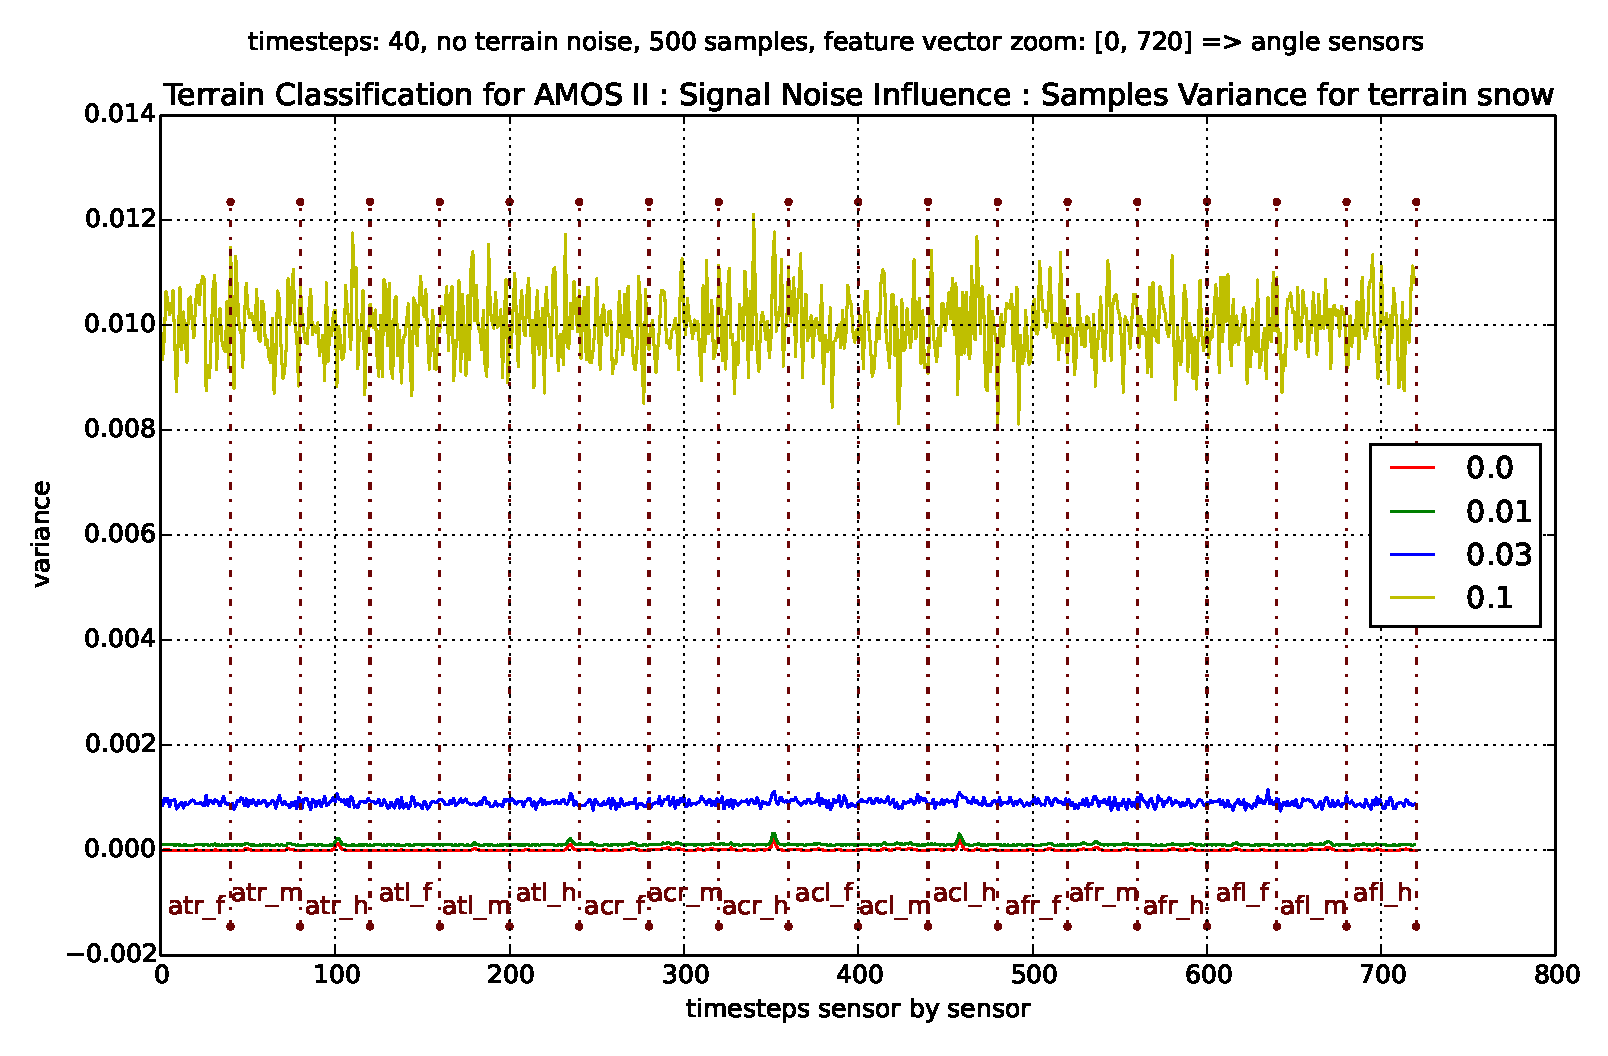
\includegraphics[width=1.0\textwidth]{sn_analysis_40_angle_snow}
%  \caption{Signal noise analysis : samples variance, terrain: snow, angle sensors}
%  \label{fig:sn_analysis_angle_snow}
%\end{figure}
%
%\begin{figure}[H]
%  \centering
%  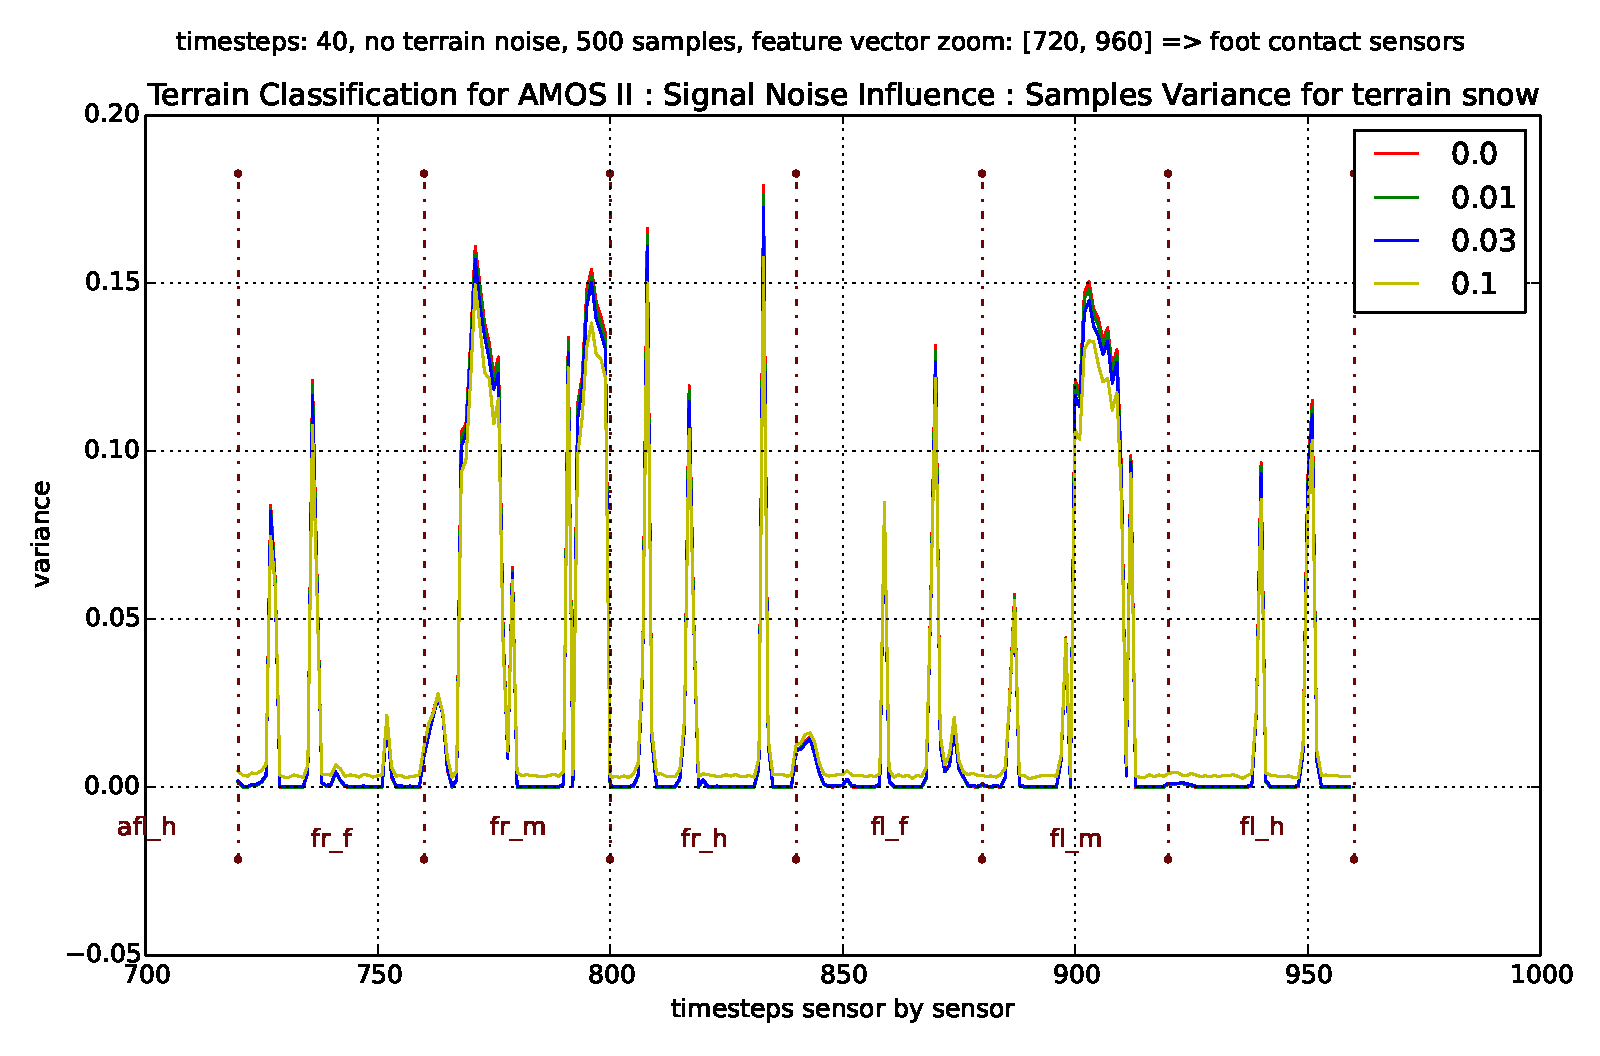
\includegraphics[width=1.0\textwidth]{sn_analysis_40_foot_contact_snow}
%  \caption{Signal noise analysis : samples variance, terrain: snow, foot contact sensors}
%  \label{fig:sn_analysis_foot_contact_snow}
%\end{figure}